%\documentclass[compress]{beamer}
\documentclass[handout]{beamer}
%\usetheme{sthlm}

%-=-=-=-=-=-=-=-=-=-=-=-=-=-=-=-=-=-=-=-=-=-=-=-=
%        LOADING BEAMER PACKAGES
%-=-=-=-=-=-=-=-=-=-=-=-=-=-=-=-=-=-=-=-=-=-=-=-=

\mode<presentation>
{
  \usetheme{Warsaw}      % or try Darmstadt, Madrid, Warsaw, ...
  \usecolortheme{default} % or try albatross, beaver, crane, ...
  \usefonttheme{serif}  % or try serif, structurebold, ...
  \setbeamertemplate{navigation symbols}{}
  \setbeamertemplate{caption}[numbered]
}

%\usepackage{
%booktabs,
%datetime,
%dtklogos,
%graphicx,
%multicol,
%pgfplots,
%ragged2e,
%tabularx,
%tikz,
%wasysym
%}

%\pgfplotsset{compat=1.8}

\usepackage{times}
\usepackage[utf8]{inputenc}
\usepackage[T1]{fontenc}
\usepackage{xcolor}
\usepackage{listings}

\usepackage{amssymb}
\usepackage{amsmath}

\usepackage{pdfpages}
\usepackage{hyperref}

\usepackage {tikz}
\usetikzlibrary {positioning}
%\usepackage {xcolor}
\definecolor {processblue}{cmyk}{0.96,0,0,0}

\definecolor{mygreen}{rgb}{0,0.6,0}
\definecolor{mygray}{rgb}{0.5,0.5,0.5}
\definecolor{mymauve}{rgb}{0.1,0.6,0.78}

\lstset{ %
  backgroundcolor=\color{white},   % choose the background color; you must add \usepackage{color} or \usepackage{xcolor}
  basicstyle=\footnotesize,        % the size of the fonts that are used for the code
  breakatwhitespace=false,         % sets if automatic breaks should only happen at whitespace
  breaklines=true,                 % sets automatic line breaking
  captionpos=b,                    % sets the caption-position to bottom
  commentstyle=\color{mygreen},    % comment style
  deletekeywords={...},            % if you want to delete keywords from the given language
  escapeinside={\%*}{*)},          % if you want to add LaTeX within your code
  extendedchars=true,              % lets you use non-ASCII characters; for 8-bits encodings only, does not work with UTF-8
  frame=single,	                   % adds a frame around the code
  keepspaces=true,                 % keeps spaces in text, useful for keeping indentation of code (possibly needs columns=flexible)
  keywordstyle=\color{blue},       % keyword style
  language=Octave,                 % the language of the code
  otherkeywords={*,...},           % if you want to add more keywords to the set
  numbers=left,                    % where to put the line-numbers; possible values are (none, left, right)
  numbersep=5pt,                   % how far the line-numbers are from the code
  numberstyle=\tiny\color{mygray}, % the style that is used for the line-numbers
  rulecolor=\color{black},         % if not set, the frame-color may be changed on line-breaks within not-black text (e.g. comments (green here))
  showspaces=false,                % show spaces everywhere adding particular underscores; it overrides 'showstringspaces'
  showstringspaces=false,          % underline spaces within strings only
  showtabs=false,                  % show tabs within strings adding particular underscores
  stepnumber=2,                    % the step between two line-numbers. If it's 1, each line will be numbered
  stringstyle=\color{mymauve},     % string literal style
  tabsize=2,	                   % sets default tabsize to 2 spaces
  title=\lstname                   % show the filename of files included with \lstinputlisting; also try caption instead of title
}


\makeatother
\setbeamertemplate{footline}
{
  \leavevmode%
  \hbox{%
  \begin{beamercolorbox}[wd=.4\paperwidth,ht=2.25ex,dp=1ex,center]{author in head/foot}%   
    \color{gray}
    \usebeamerfont{author in head/foot}\insertshortauthor
  \end{beamercolorbox}%
  \begin{beamercolorbox}[wd=.6\paperwidth,ht=2.25ex,dp=1ex,center]{title in head/foot}%            
    \color{mymauve}
    \usebeamerfont{title in head/foot}\insertshorttitle\hspace*{3em}
    \insertframenumber{} / \inserttotalframenumber\hspace*{1ex}
  \end{beamercolorbox}}%
  \vskip0pt%
}
\makeatletter
\setbeamertemplate{navigation symbols}{}

\AtBeginSection[]{
  \begin{frame}
  \vfill
  \centering
  \begin{beamercolorbox}[sep=8pt,center,shadow=true,rounded=true]{title}
    \usebeamerfont{title}\insertsectionhead\par%
  \end{beamercolorbox}
  \vfill
  \end{frame}
}

\newcommand{\EM}{$\Omega$~}
\newcommand{\MP}{$\mathrm{P}$~}
\newcommand{\SA}{$\sigma$--\'algebra~}
\newcommand{\FF}{$\mathcal{F}$~}

\newcommand{\eg}{$\triangleright$e.g.:}
\newcommand{\MA}{\textsc{Muestra aleatoria} }
\newcommand{\PH}{\textsc{Prueba de hip\'otesis} }
\newcommand{\IC}{\textsc{Intervalo de Confianza} }
\newcommand{\VA}{\textsc{Variable aleatoria} }
\newcommand{\HN}{\textsc{hip\'otesis nula} }
\newcommand{\HA}{\textsc{hip\'otesis alternativa} }
\newcommand{\hn}{H$_0$ }
\newcommand{\ha}{H$_1$ }
 
                
%-=-=-=-=-=-=-=-=-=-=-=-=-=-=-=-=-=-=-=-=-=-=-=-=
%        LOADING TIKZ LIBRARIES
%-=-=-=-=-=-=-=-=-=-=-=-=-=-=-=-=-=-=-=-=-=-=-=-=

%\usetikzlibrary{
%backgrounds,
%mindmap
%}

%-=-=-=-=-=-=-=-=-=-=-=-=-=-=-=-=-=-=-=-=-=-=-=-=
%        BEAMER OPTIONS
%-=-=-=-=-=-=-=-=-=-=-=-=-=-=-=-=-=-=-=-=-=-=-=-=

%-=-=-=-=-=-=-=-=-=-=-=-=-=-=-=-=-=-=-=-=-=-=-=-=
%        DEFINITIONS
%-=-=-=-=-=-=-=-=-=-=-=-=-=-=-=-=-=-=-=-=-=-=-=-=
 
\theoremstyle{plain}

\newtheorem{teorema}{Teorema}[section]
\newtheorem{prop}[teorema]{Proposici\'on}
\newtheorem{lema}[teorema]{Lema}
\newtheorem{corolario}[teorema]{Corolario}

\theoremstyle{definition}
\newtheorem{definicion}[teorema]{Def./}
\newtheorem{ejemplo}[teorema]{$\triangleright$ e.g.}
\newtheorem{pregunta}[teorema]{?}
%\newtheorem{ejercicio}[teorema]{Ejercicio}

\theoremstyle{remark}
%\newtheorem{nota}[teorema]{Nota}

\newtheorem{problema}{Problema}[section]
\newtheorem{ejercicio}{Ejercicio}[section]
\newtheorem{aplicacion}{Aplicación}[section]
%\theoremstyle{remark}
\newtheorem{observacion}{Observación}[section]
\newtheorem{nota}[teorema]{Nota}               
 
%\setbeameroption{show notes}

%-=-=-=-=-=-=-=-=-=-=-=-=-=-=-=-=-=-=-=-=-=-=-=-=
%        BEAMER COMMANDS
%-=-=-=-=-=-=-=-=-=-=-=-=-=-=-=-=-=-=-=-=-=-=-=-=


%-=-=-=-=-=-=-=-=-=-=-=-=-=-=-=-=-=-=-=-=-=-=-=-=
%
%	PRESENTATION INFORMATION
%
%-=-=-=-=-=-=-=-=-=-=-=-=-=-=-=-=-=-=-=-=-=-=-=-=
\setbeamerfont{structure}{shape=\itshape, series=\bfseries}
\setbeamerfont{frametitle}{shape=\itshape,size=\normalsize}
\setbeamerfont{alerted text}{shape=\itshape, series=\bfseries}
\setbeamercolor{alerted text}{fg=black}

 
\author[]{Time series analysis}
\title[]{\textbf{Astrometría 2017}}
\date {\tiny{04 Dic. 2017}}
\institute[]{}%
\subject{Astrometría 2017}


\begin{document}
\author{OTHER 2017}
\title{Simulaciones de comunicaciones entre ETI}
\maketitle

\footnotesize


\section{Introducci\'on}


%_________________________________________________________________________
\section{Simulaciones MonteCarlo de la ecuación de Drake}

\begin{frame}\frametitle{Forgan 2009, IJA, 8, 121}
%{{{
\centering

Title: A numerical testbed for hypotheses of extraterrestrial life and intelligence

\

Authors:	Forgan, D. H.

\

Affiliation:	AA(Scottish Universities Physics Alliance (SUPA), Institute for Astronomy, University of Edinburgh, Royal Observatory Edinburgh, Blackford Hill, Edinburgh EH9 3HJ, UK dhf@roe.ac.uk)

\

Publication:	International Journal of Astrobiology, Volume 8, Issue 2, p. 121-131
\end{frame}%}}}


\section{Simulaciones de comunicaciones en una galaxia}

\begin{frame}\frametitle{Idea}
%{{{

   Dado que los factores que intervienen en la ecuación de Drake son
   muy inciertos, la propuesta consiste en evitar el uso de la
   ecuación y explorar un espacio de hipótesis.

   \ 

   La única observación que se puede usar es el tiempo durante el cual
   se llevaron a cabo proyectos SETI y no se encontró nada.

\end{frame}%}}}
         
\begin{frame}\frametitle{Aproximación de eventos discretos}
%{{{

   La \alert{simulación por eventos discretos} es una aproximación que
   consiste en codificar el comportamiento de sistemas complejos 
   como una secuencia de eventos bien definidos y ordenados.

   \

   Un \alert{evento} es un cambio específico en el estado del sistema a un
   determinado instante de tiempo.

   \

   Este enfoque involucra:

   \begin{itemize}
      \item Cambios en el sistema en el tiempo, relacionados
         por una sucesión de eventos
      \item Seguimiento de un conjunto de variables
      \item Definición del estado inicial y final
      \item Un método que registre el avance del tiempo
      \item Registro de una sucesión de eventos
   \end{itemize}                        
  
\end{frame}%}}}
              


%_________________________________________________________________________
\subsection{Variables de la simulación}
 
\begin{frame}\frametitle{Definiciones}
%{{{

   \begin{description}
      \item[CETI]  Communicating Extraterrestrial Inteligence
      \item[FCS] First Contact Surface 
      \item[LCS] Last Contact Surface 
      \item[$\tau_{ceti}$] Tiempo medio entre la aparición de CETIs
      \item[$\tau_{a}$] Vida media de una CETI.  Periodo promedio de tiempo
         durante el cual la CETI está activa
      \item[$D_{max}$] Máxima distancia a la cual una CETI es capaz de
         transmitir o recibir mensajes
   \end{description}

\end{frame}%}}}
 
\begin{frame}\frametitle{Hipótesis}
%{{{

   En la primera aproximación:

   \begin{itemize}
      \item No hay una ventana temporal que favorezca la aparición de
         CETIs.   Es igualmente probable dentro del periodo de tiempo
         considerado, que es mucho mayor al tiempo medio entre
         surgimiento de nuevas CETIs
      \item Las condiciones para la aparición de CETIs son homogéneas
         en toda la zona habitable galáctica
      \item El medio de comunicación viaja a la velocidad de la luz
      \item La capacidad de emisión y recepción de mensajes está
         limitada por la misma distancia máxima
      \item La distribución en el tiempo de la aparición de CETIs es
         un proceso de Poisson
      \item La distribución en la vida media de CETIs es exponencial
   \end{itemize}

\end{frame}%}}}

\begin{frame}\frametitle{Variables de la simulación}
%{{{

   \begin{itemize}
      \item Posición de las estrellas
      \item Tiempo de inicio de la capacidad de comunicación
      \item Tiempo de finalización de la capacidad de comunicación
      \item Número de CETIs en contacto causal con otras CETIs
      \item Número de CETIs
   \end{itemize}

\end{frame}%}}}
 
\begin{frame}\frametitle{Variables de inicialización}
%{{{


   Variables tomadas de la bibliografía:

   \begin{itemize}
      \item Zona habitable galáctica
      \item Número medio de CETIs (Ec. de Drake)
   \end{itemize}

   \vspace{1cm}

   Variables a explorar:

    \begin{itemize}
      \item Número medio de CETIs por unidad de tiempo en toda la
         galaxia
      \item Vida media de una CETI
   \end{itemize}
 

\end{frame}%}}}
                         
\begin{frame}\frametitle{Objetivos}
%{{{

   En función de $\tau_{CETI}$, $\tau_{a}$ y $D_{max}$, y bajo las
   hipótesis propuestas,

   \begin{itemize}
      \item Cuál es el número estimado de CETIs que alguna vez reciben un
         mensaje de otra CETI?
      \item Cuál es el número medio de CETIs que alguna vez reciben un
         mensaje de otra CETI y envían un mensaje que llega a destino
         durante la etapa activa de la CETI que emitión el mensaje
         original?
      \item Cuál es el tiempo promedio que debería esperar una CETI
         para recibir un mensaje de otra CETI?
   \end{itemize}

\end{frame}%}}}
                    
\begin{frame}\frametitle{Refinamiento en el planteo de las hipótesis}
%{{{

   \begin{itemize}
      \item La $D_{max}$ es diferente para diferentes CETIs
      \item La distribución de $D_{max}$ es una ley de potencias: Las
         emisiones potentes son poco probables y las poco potentes son
         más probables
      \item Las probabilidades del surgimiento de CETIs varía en
         función de la distancia al centro de la galaxia
      \item Factor de eficiencia: si los mensajes son intermitentes,
         salvo que se monitoree el todo el cielo de manera constante,
         puede pasar que los mensajes pasen sin ser detectados.
   \end{itemize}

\end{frame}%}}}
                        
\begin{frame}\frametitle{Factor espiritual}
%{{{

   Como refinamiento de las hipótesis de la simulación, se puede
   además explorar el rol del factor S:

   \begin{itemize}
      \item El contenido del mensaje depende del factor S.          
      \item Esto puede afectar la vida media de otras CETI que reciban el mensaje.
      \item La vida media de una CETI depende del factor S
   \end{itemize}

\end{frame}%}}}
                     
\begin{frame}\frametitle{Posibles implicaciones}
%{{{

   \begin{itemize}
      \item Análisis del método de comunicación: isotrópico, colimado,
         accidental
      \item Naturaleza del transporte del mensaje: radiación
         electromagnética u otros
      \item Efectos de fenómenos de alineación (tránsitos)
      \item Marcadores energéticos
      \item Marcadores espirituales
      \item Uso de estrellas como amplificadores o fuentes
   \end{itemize}

\end{frame}%}}}
 
                
%_________________________________________________________________________
\subsection{Implementación de la simulación}


\begin{frame}\frametitle{Modelo gráfico}
%{{{
\centering
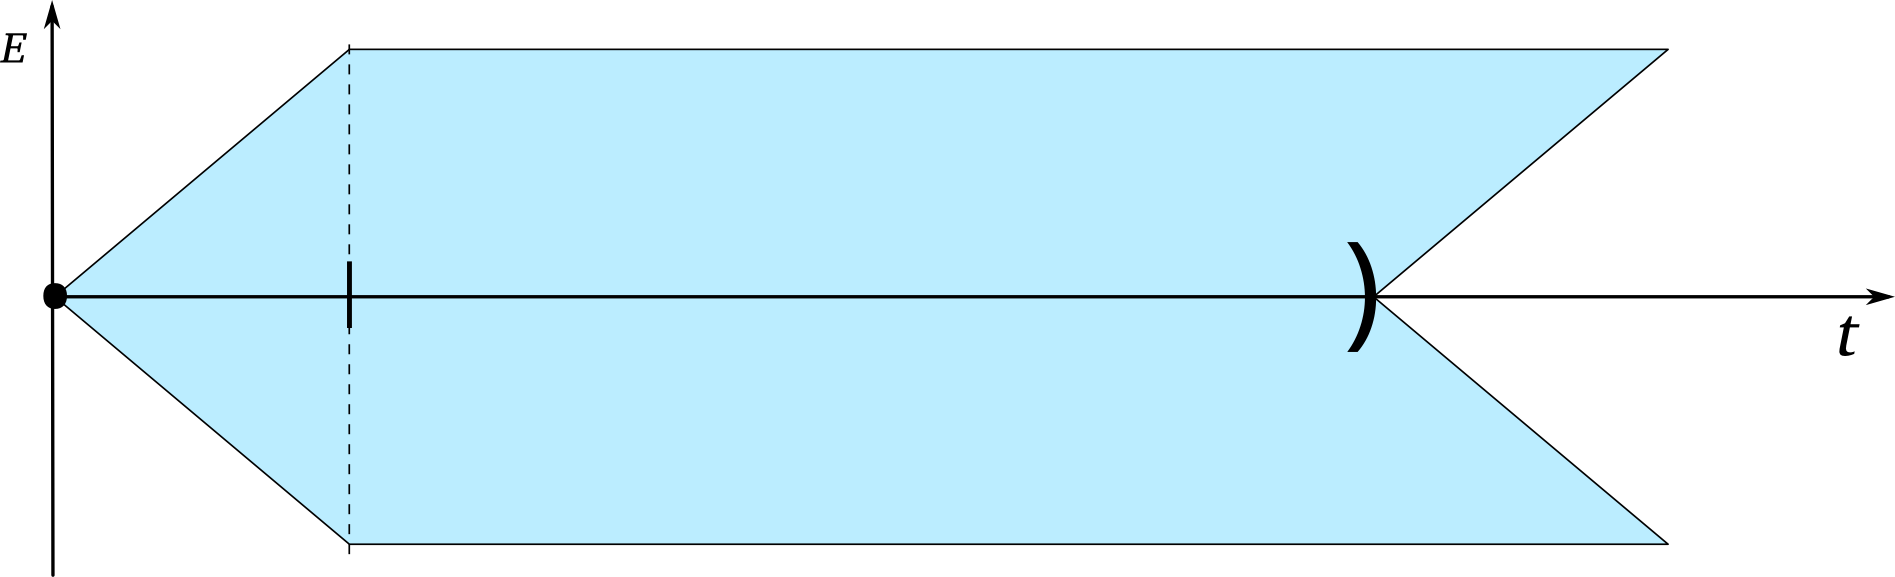
\includegraphics[width=0.9\textwidth]{text4616-5-8-3b.png}
\end{frame}%}}}

\begin{frame}\frametitle{Modelo gráfico}
%{{{
\centering
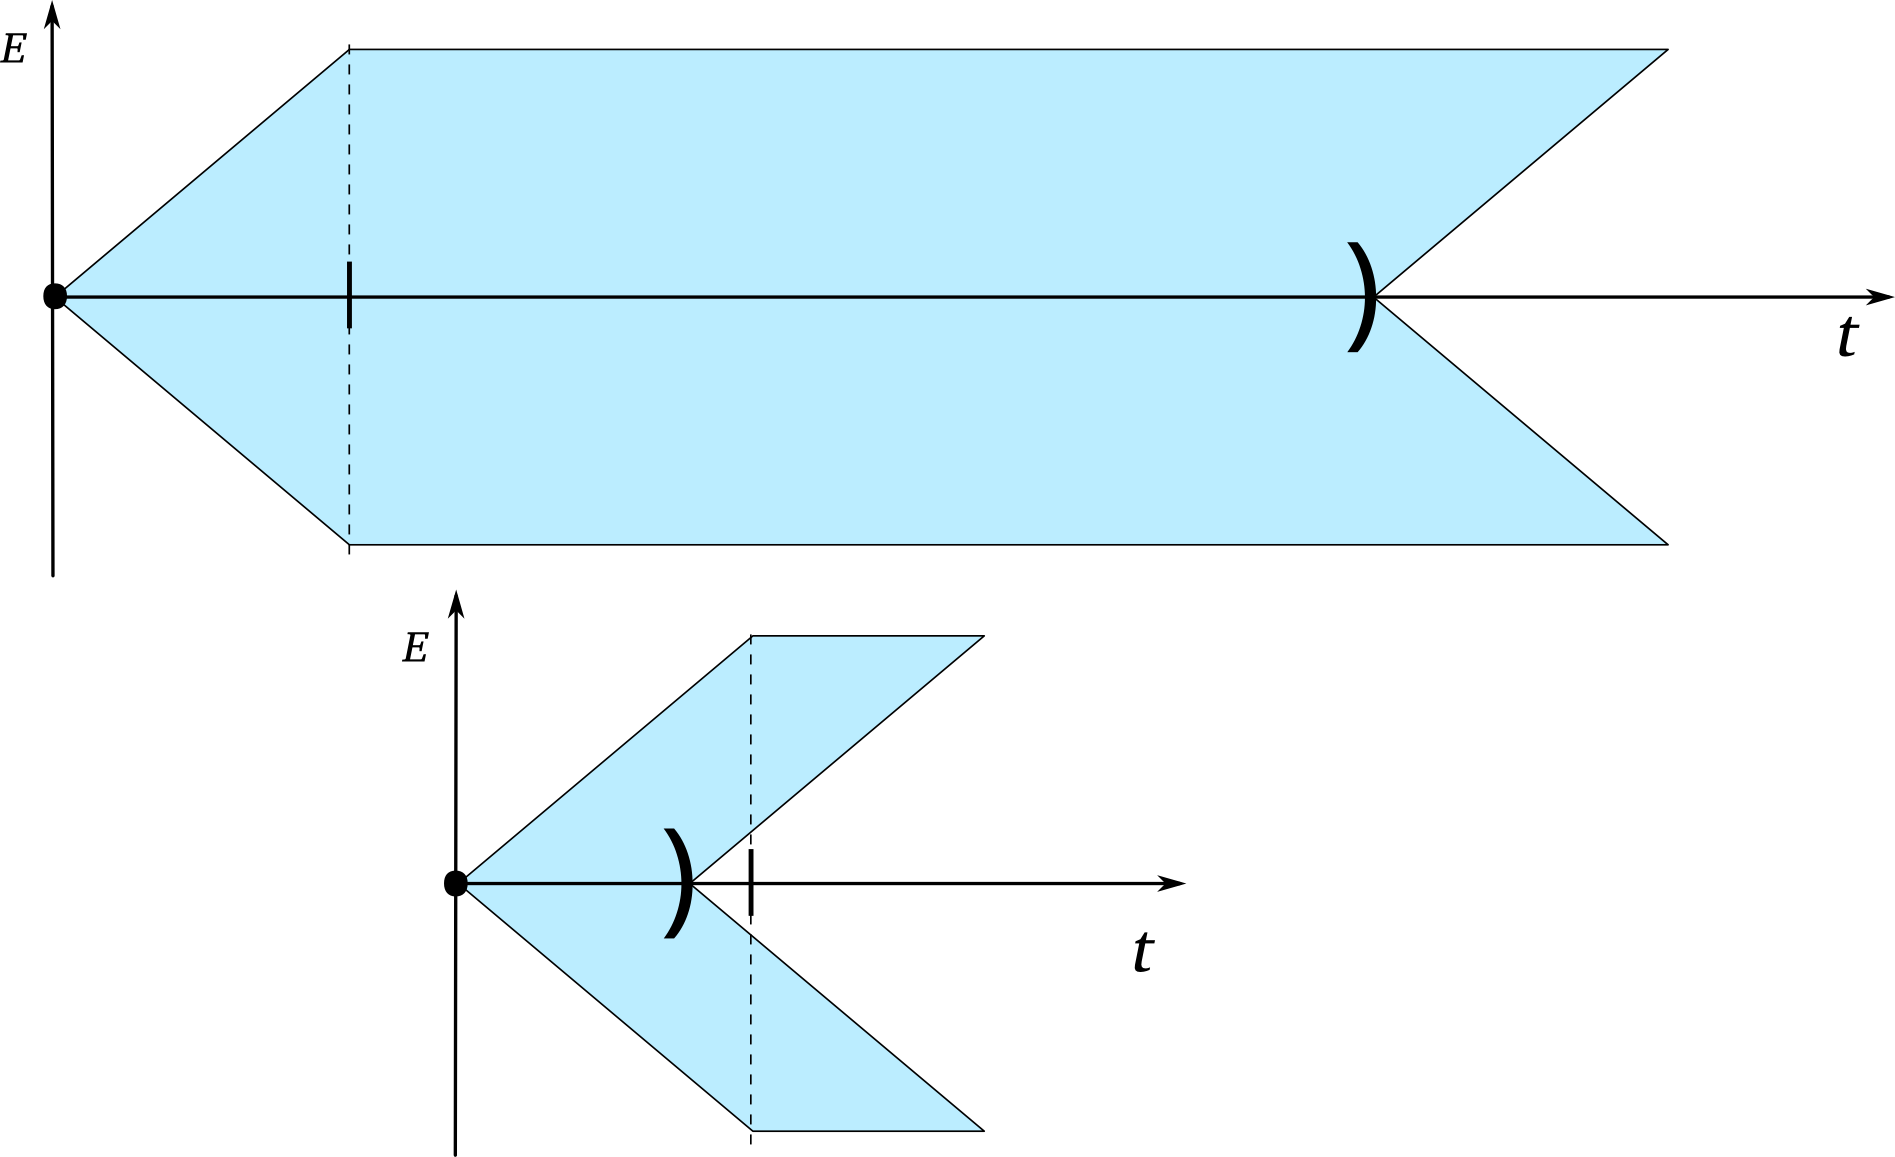
\includegraphics[width=0.9\textwidth]{text4616-5-8-3.png}
\end{frame}%}}}

\begin{frame}\frametitle{Modelo gráfico}
%{{{
\centering
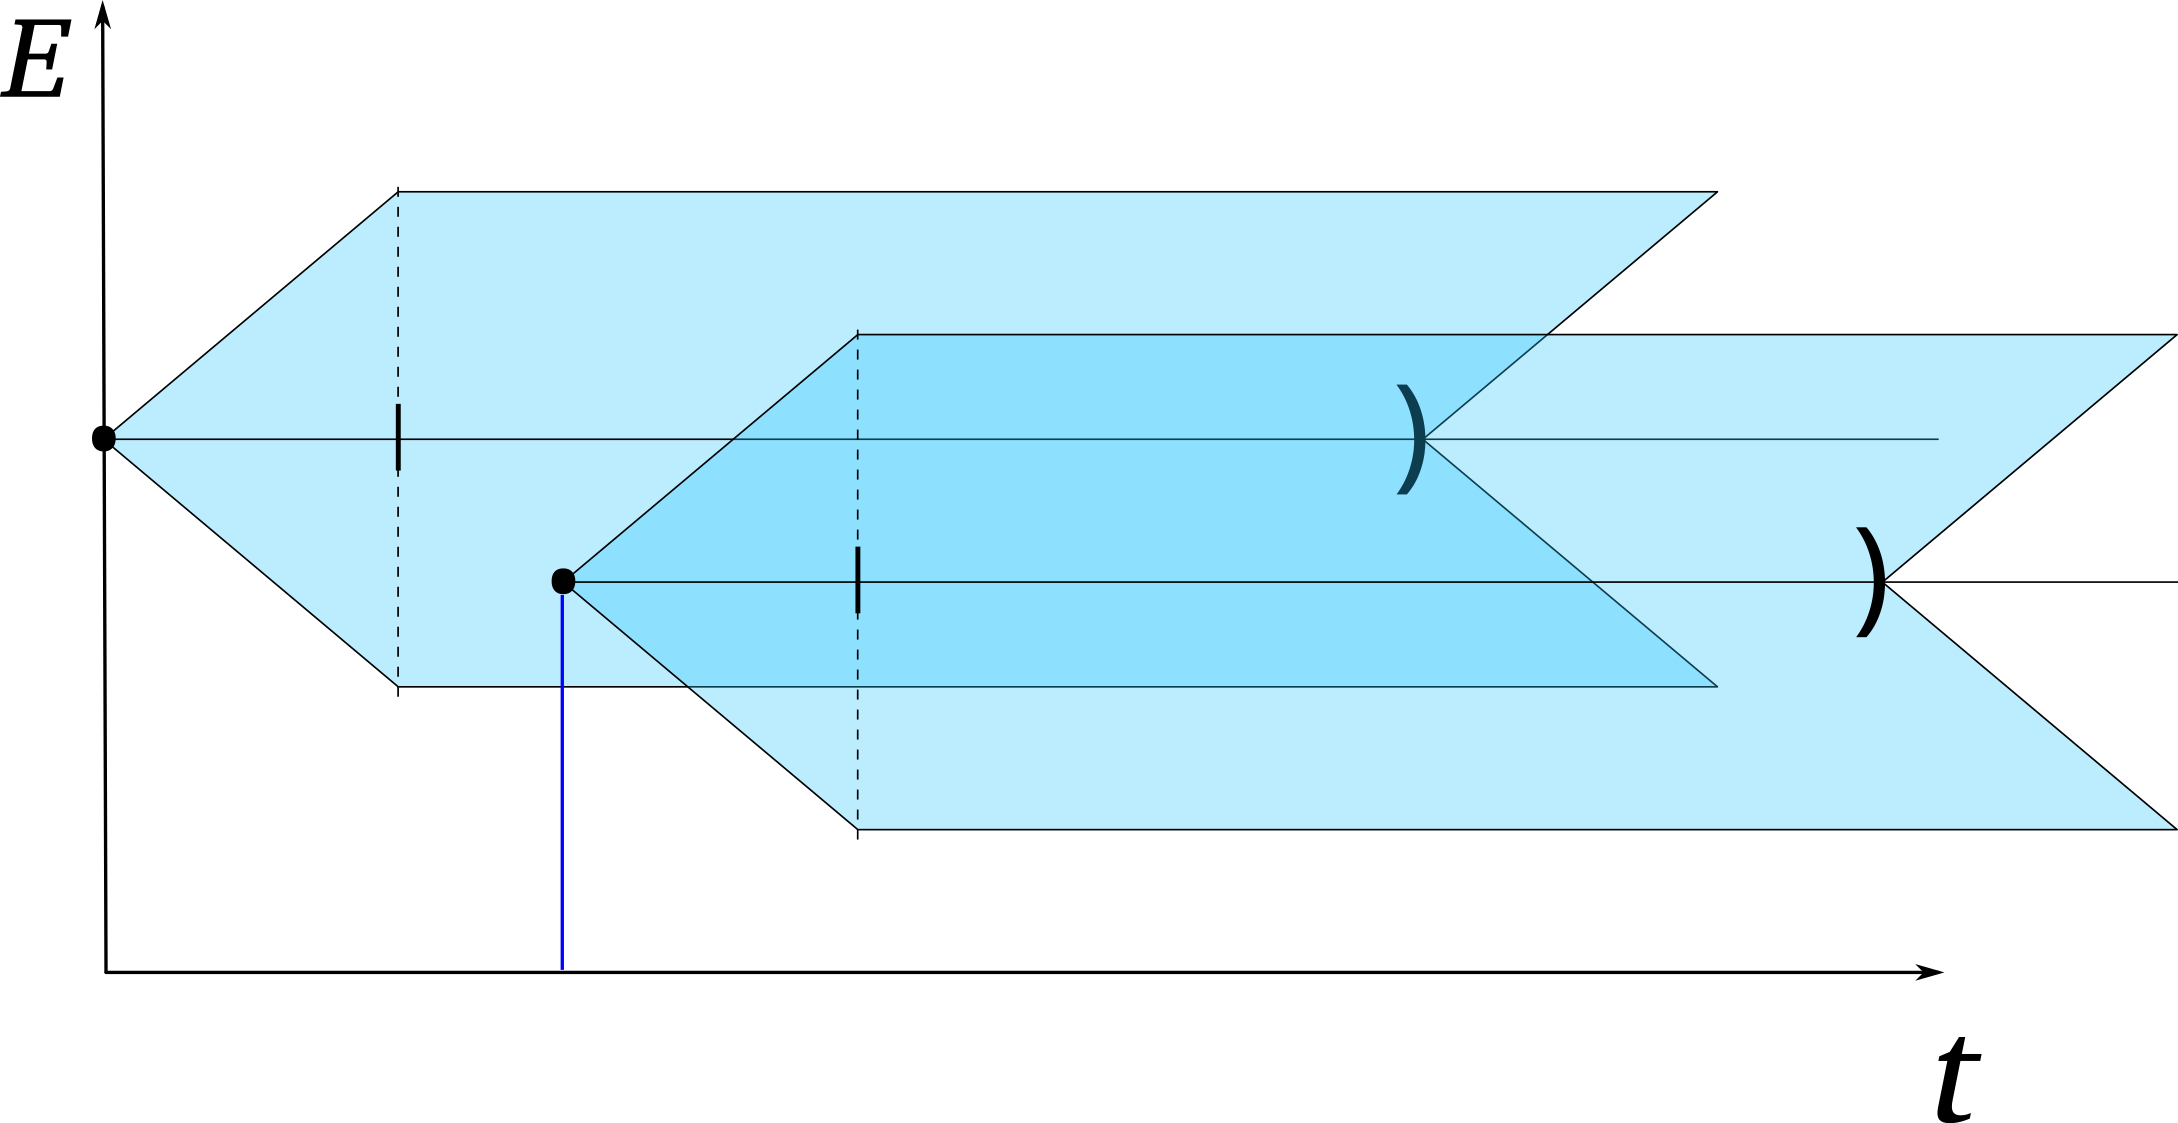
\includegraphics[width=0.9\textwidth]{text4616-5.png}
\end{frame}%}}}

\begin{frame}\frametitle{Modelo gráfico para la evolución temporal de
%{{{
   una CETI}
\centering
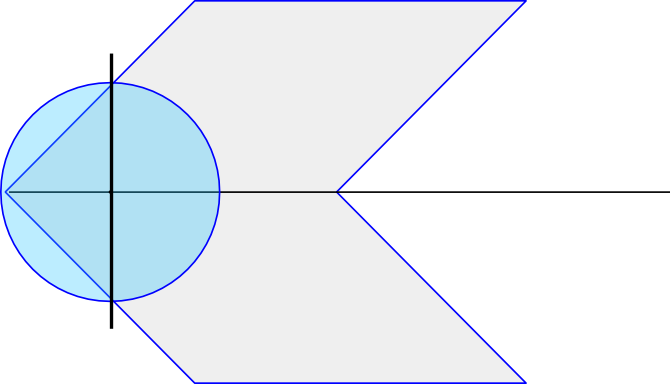
\includegraphics[width=0.5\textwidth]{g5090.png}
\end{frame}%}}}

\begin{frame}\frametitle{Modelo gráfico para la evolución temporal de
%{{{
   una CETI}
\centering
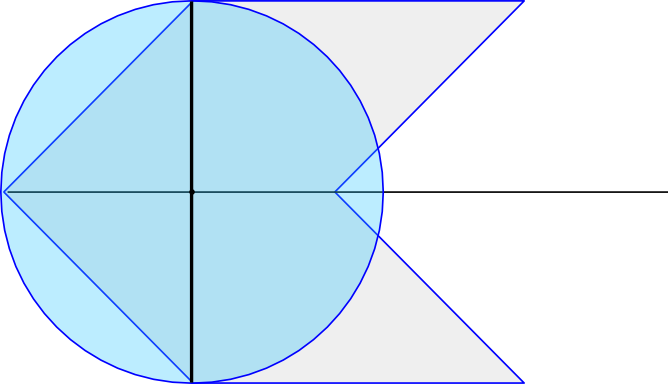
\includegraphics[width=0.5\textwidth]{g5098.png}
\end{frame}%}}}

\begin{frame}\frametitle{Modelo gráfico para la evolución temporal de
%{{{
   una CETI}
\centering
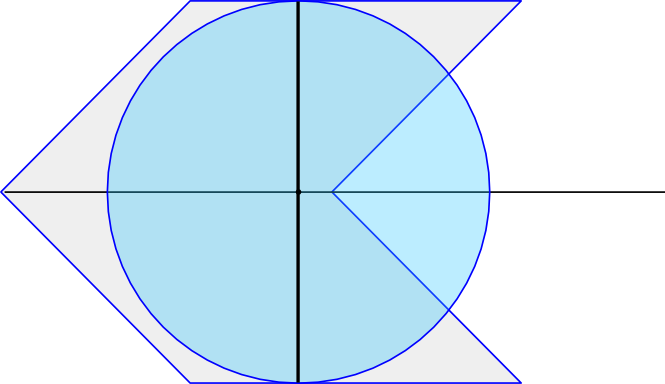
\includegraphics[width=0.5\textwidth]{g5106.png}
\end{frame}%}}}

\begin{frame}\frametitle{Modelo gráfico para la evolución temporal de
%{{{
   una CETI}
\centering
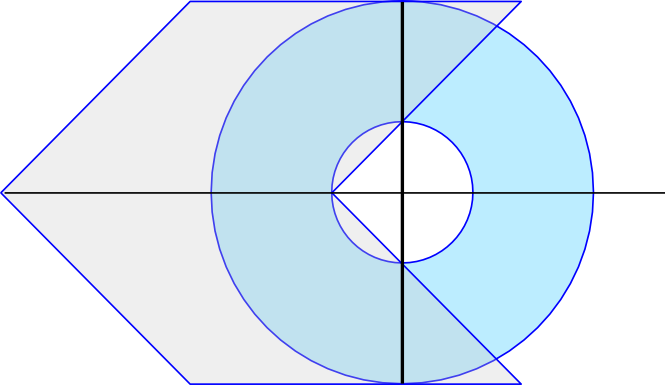
\includegraphics[width=0.5\textwidth]{g5114.png}
\end{frame}%}}}

\begin{frame}\frametitle{Modelo gráfico para la evolución temporal de
%{{{
   una CETI}
\centering
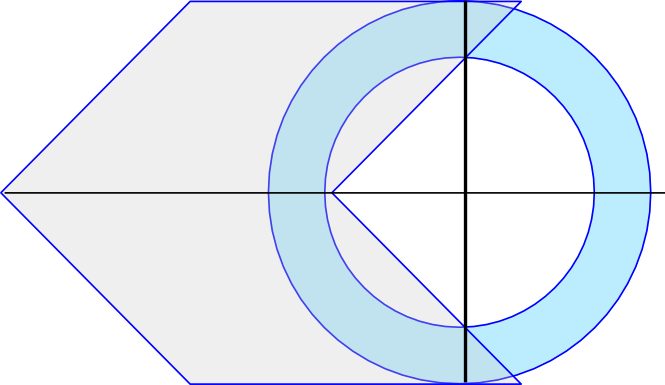
\includegraphics[width=0.5\textwidth]{g5120.png}
\end{frame}%}}}

\begin{frame}\frametitle{Modelo gráfico para la comunicación}
%{{{
\centering
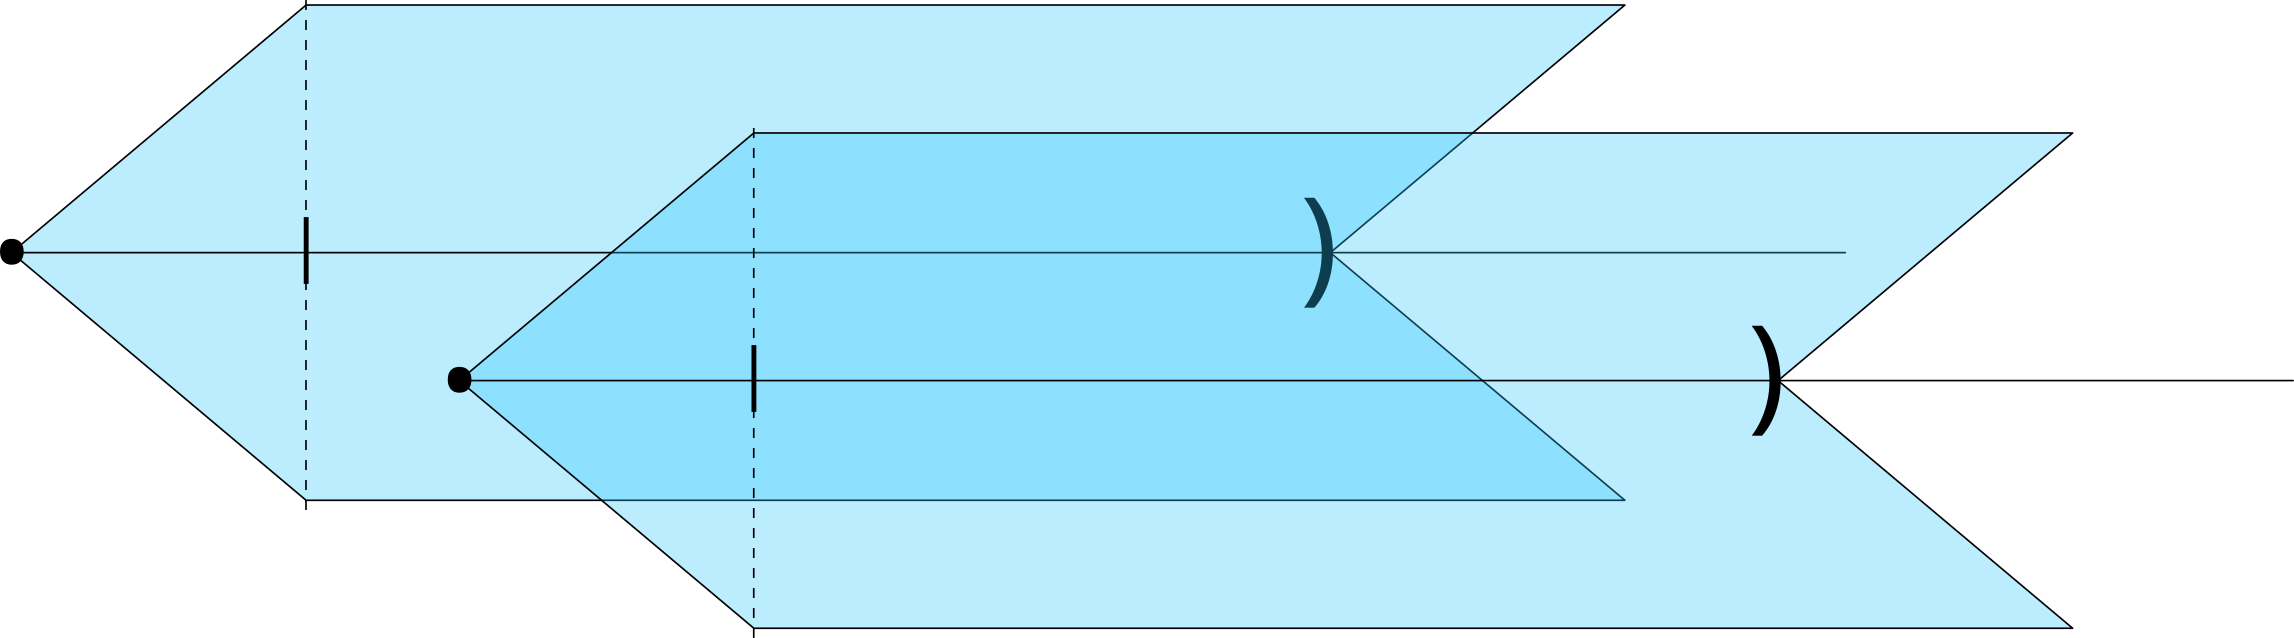
\includegraphics[width=0.8\textwidth]{g5331.png}
\end{frame}%}}}

\begin{frame}\frametitle{Modelo gráfico para la comunicación}
%{{{
\centering
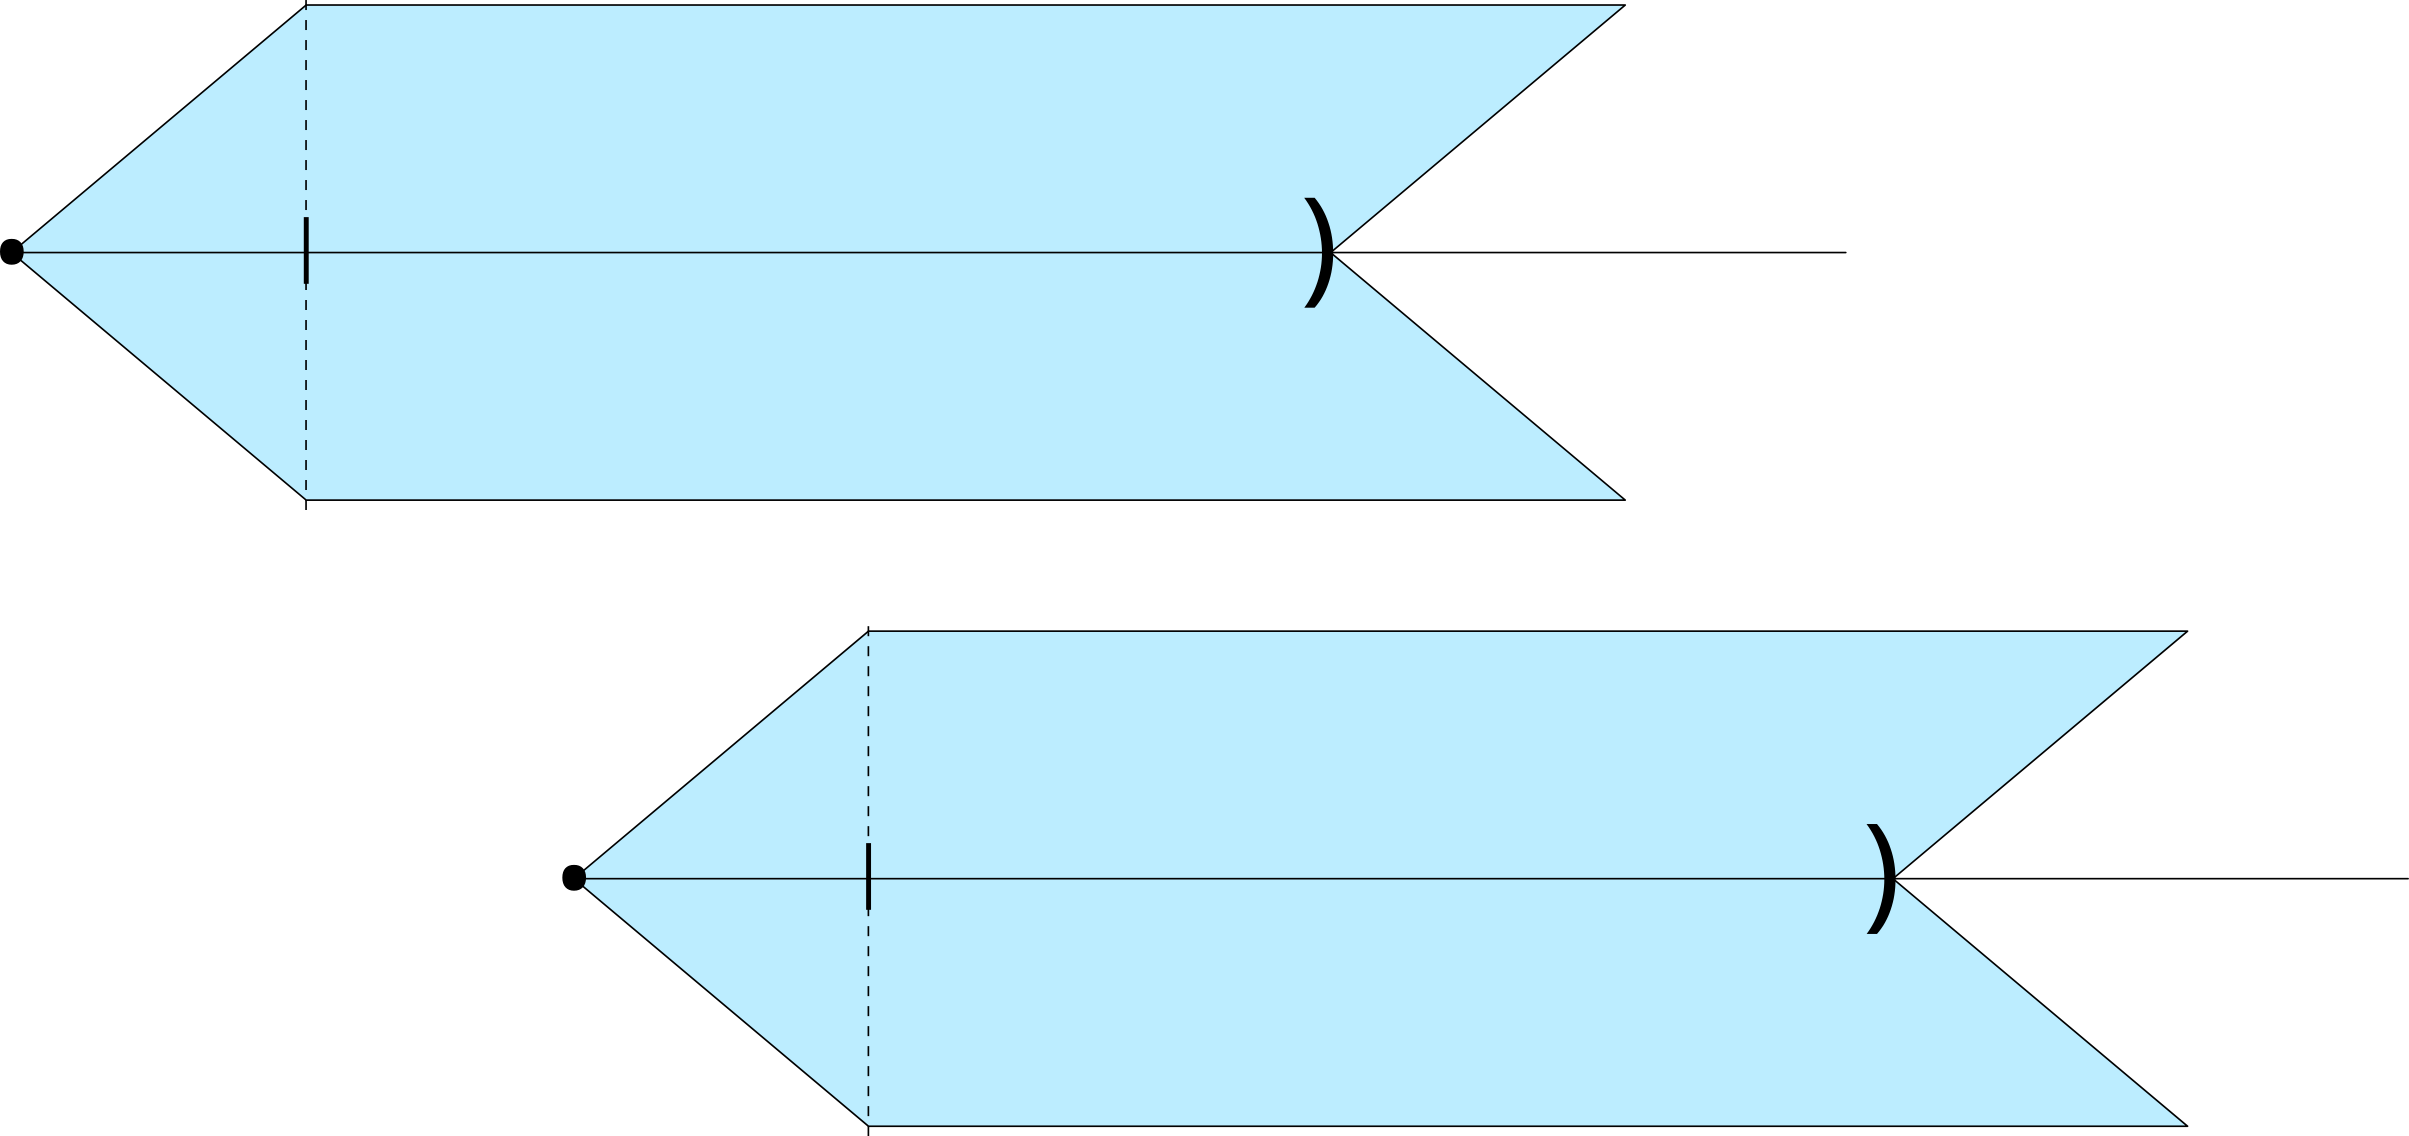
\includegraphics[width=0.8\textwidth]{g5459.png}
\end{frame}%}}}

\begin{frame}\frametitle{Modelo gráfico para la comunicación}
%{{{
\centering
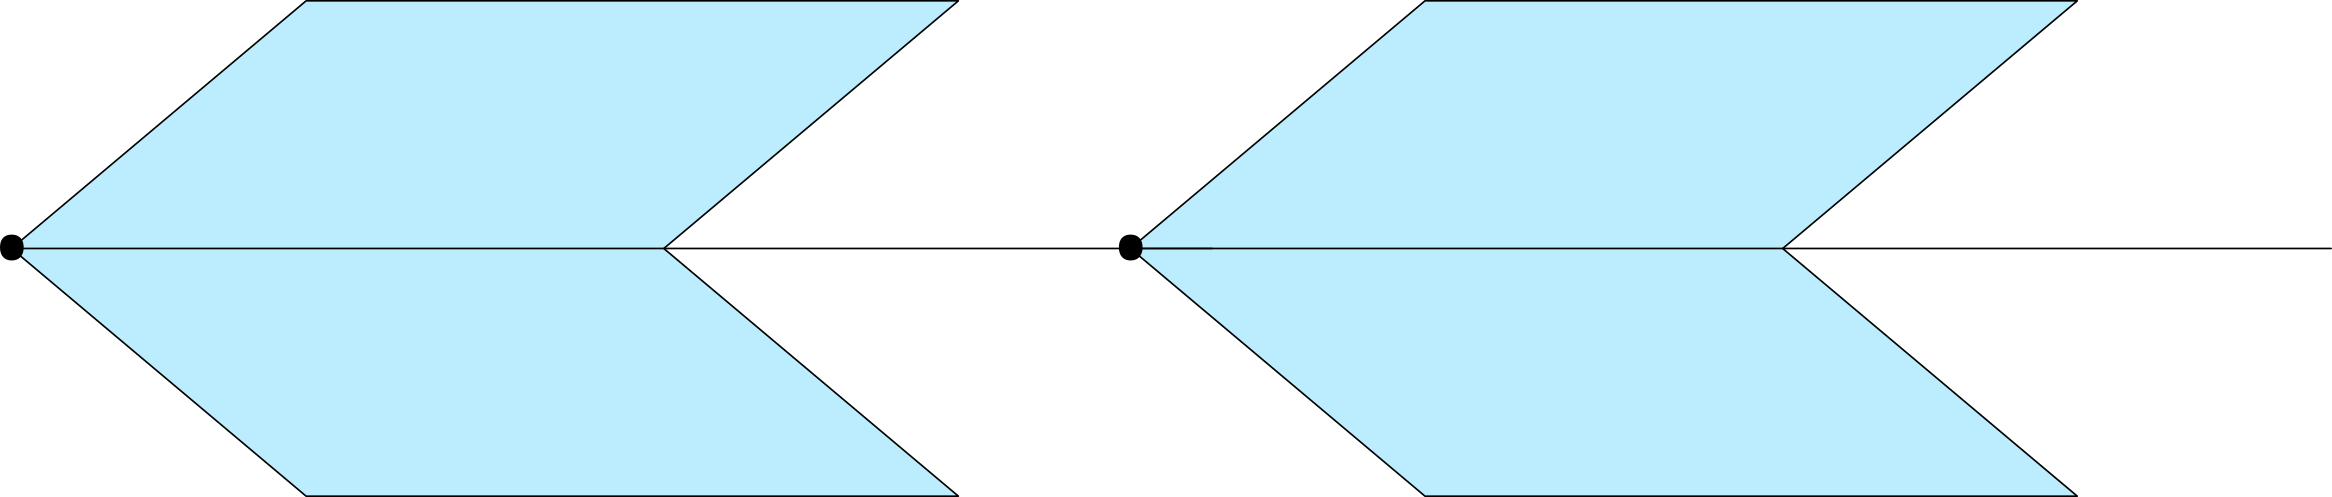
\includegraphics[width=0.8\textwidth]{g5539.png}
\end{frame}%}}}

\begin{frame}\frametitle{Modelo gráfico para la comunicación}
%{{{
\centering
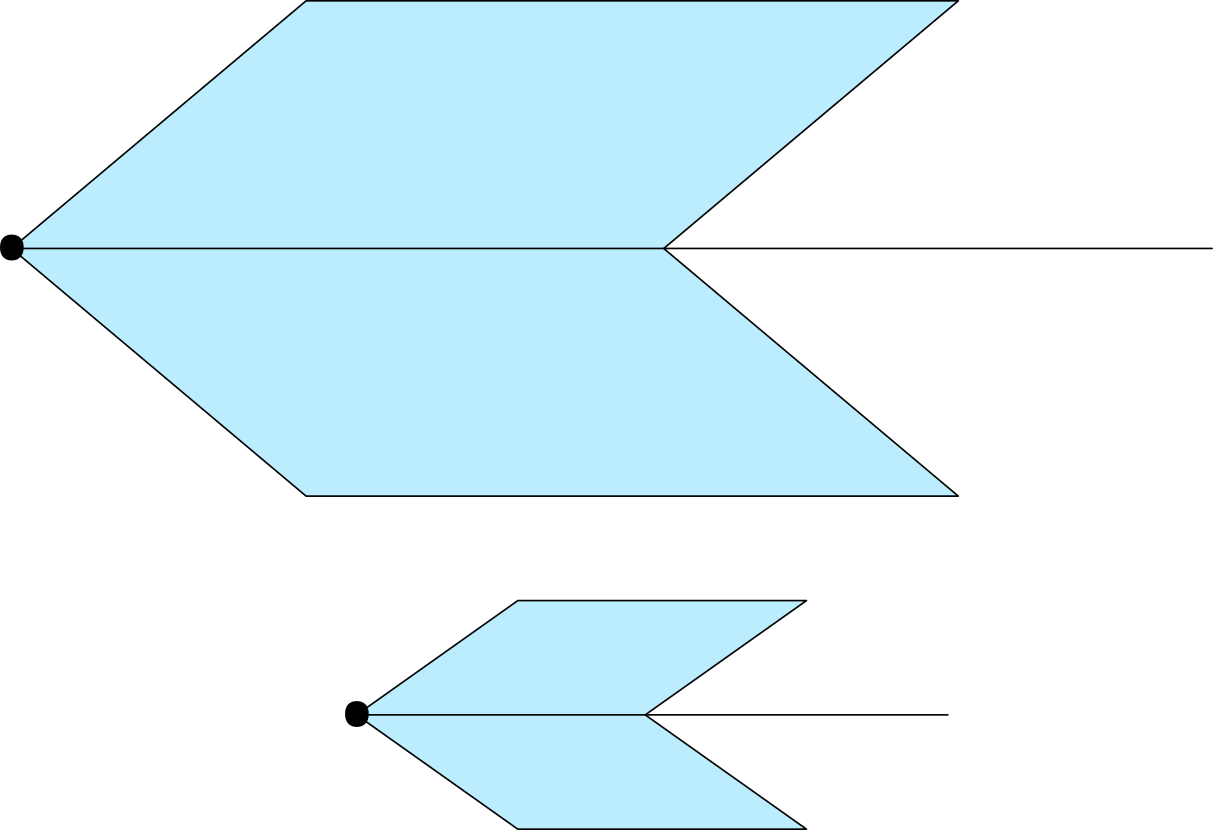
\includegraphics[width=0.8\textwidth]{g5579.png}
\end{frame}%}}}

\begin{frame}\frametitle{Modelo gráfico para el análisis espacial}
%{{{
\centering
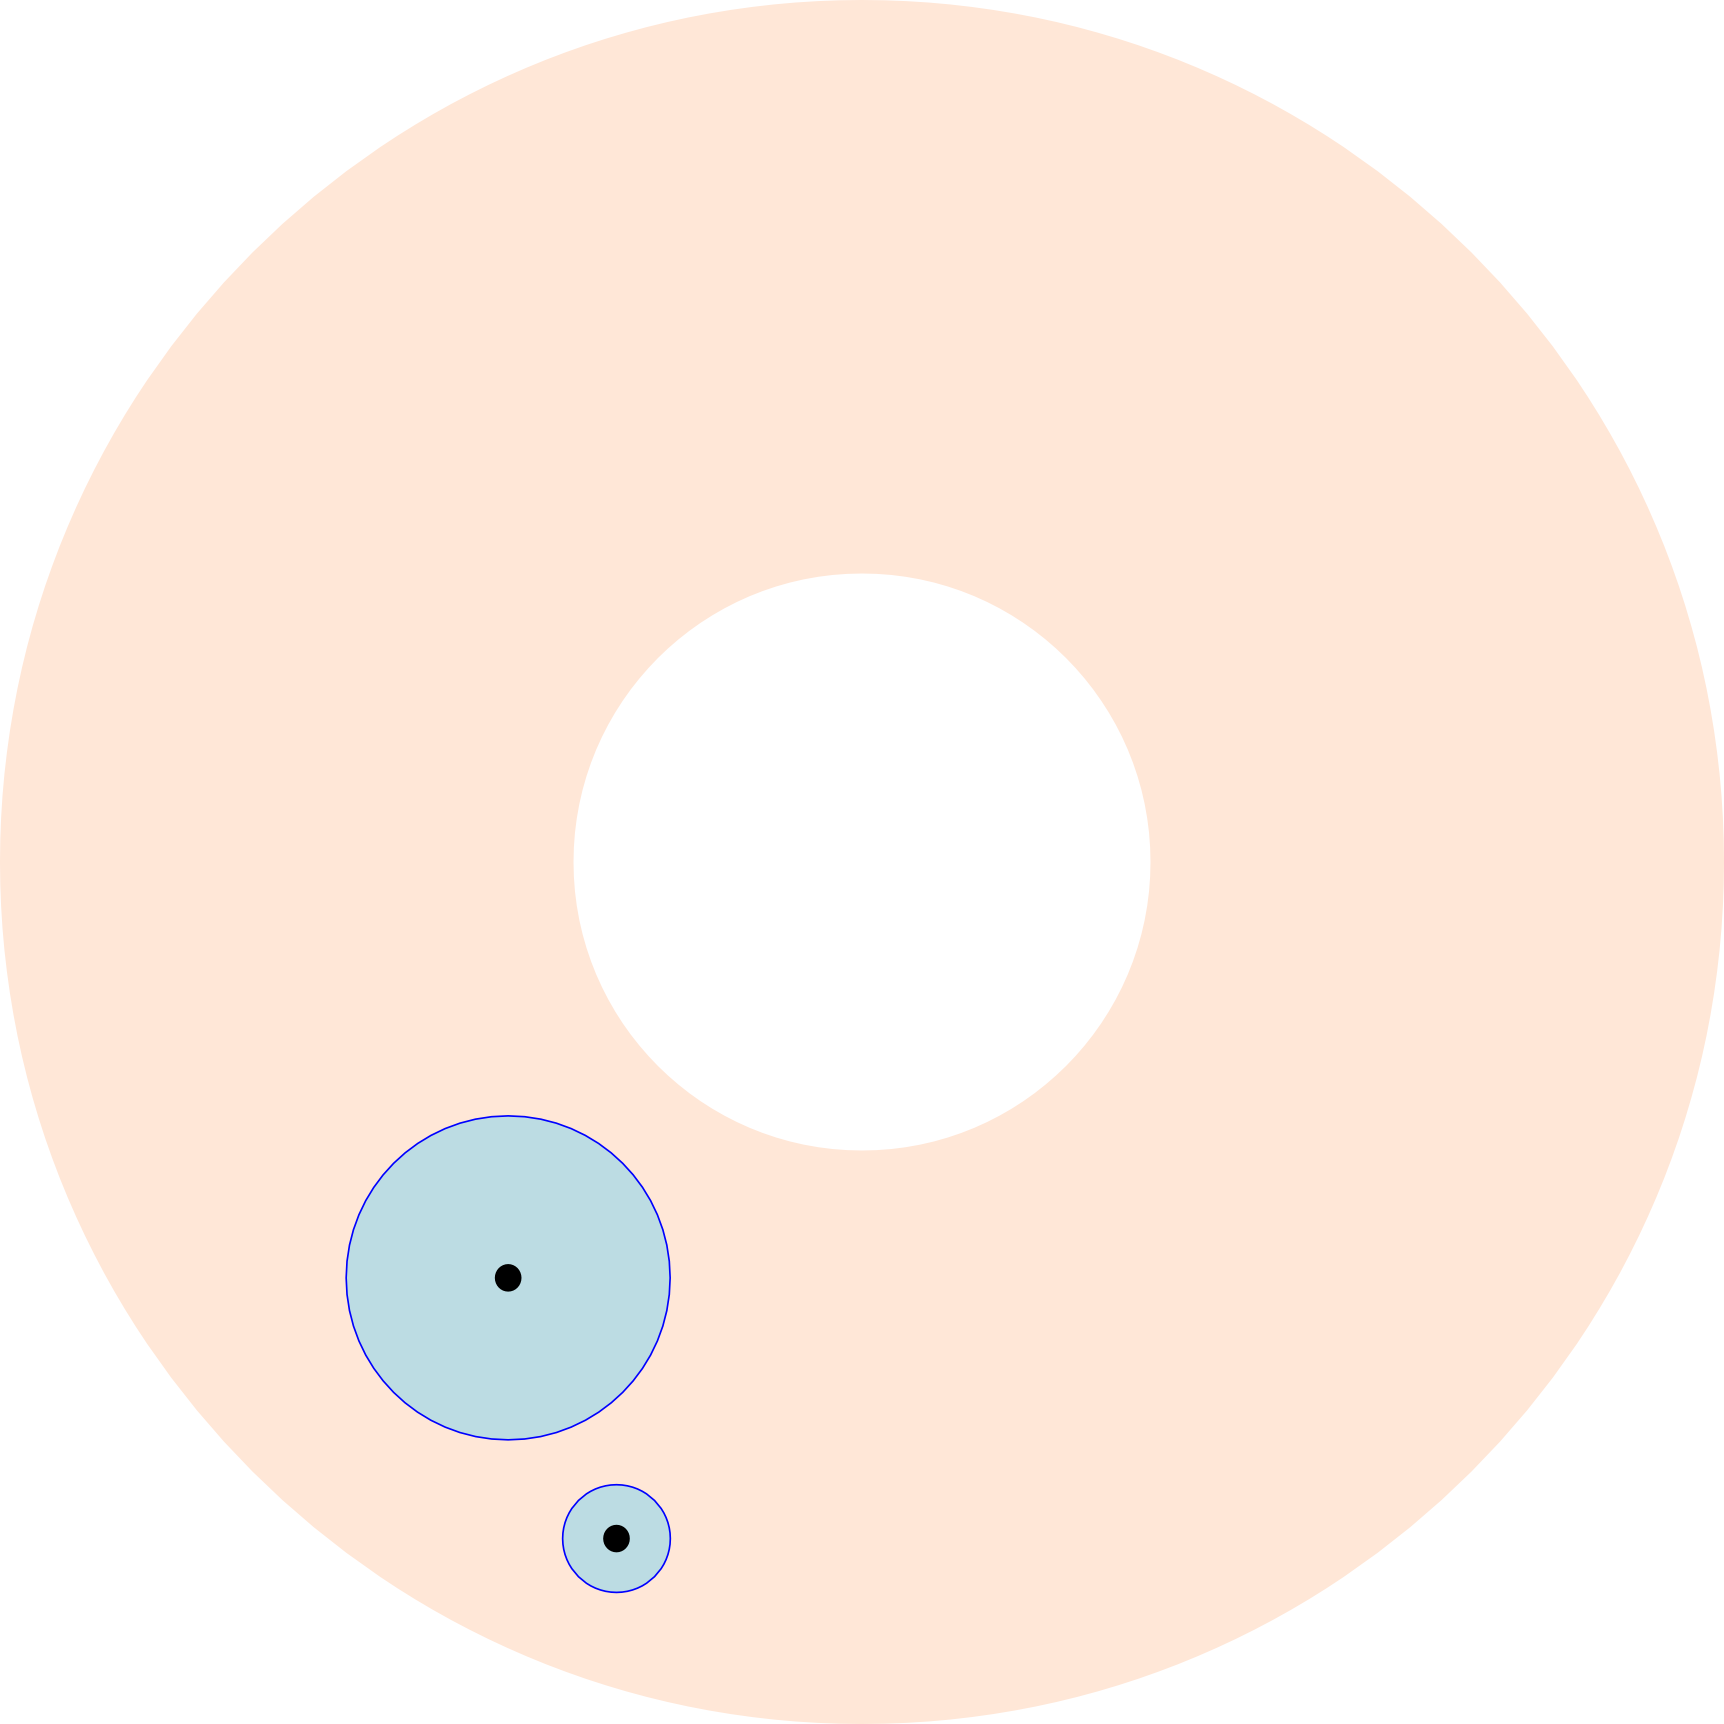
\includegraphics[width=0.5\textwidth]{path5812.png}
\end{frame}%}}}

\begin{frame}\frametitle{Modelo gráfico para el análisis espacial}
%{{{
\centering
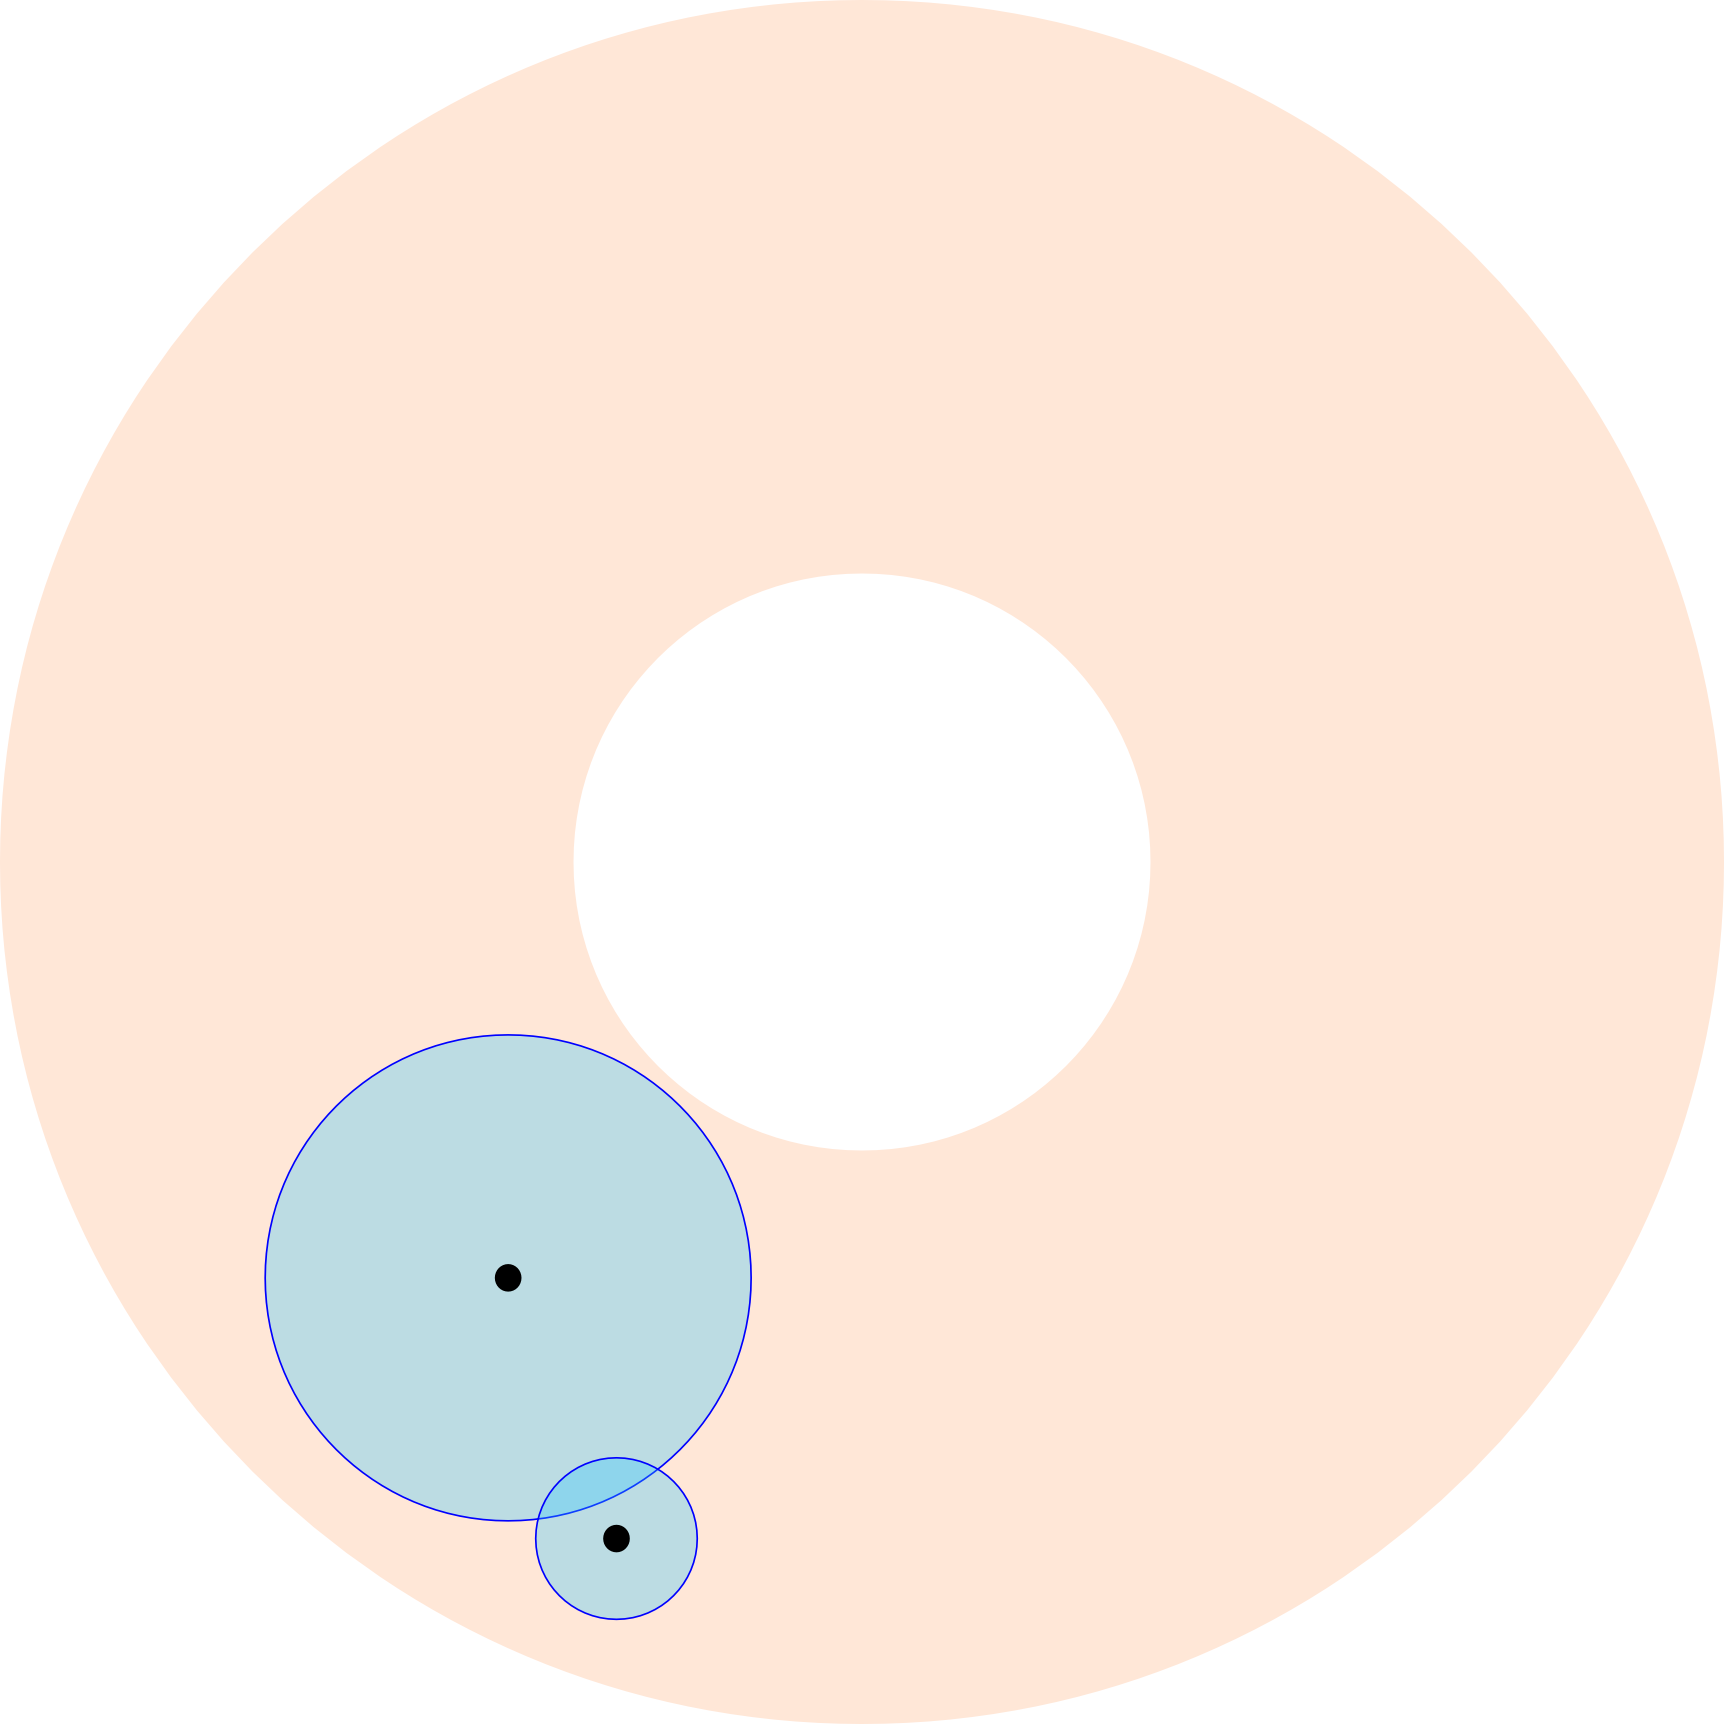
\includegraphics[width=0.5\textwidth]{path5813.png}
\end{frame}%}}}

\begin{frame}\frametitle{Modelo gráfico para el análisis espacial}
%{{{
\centering
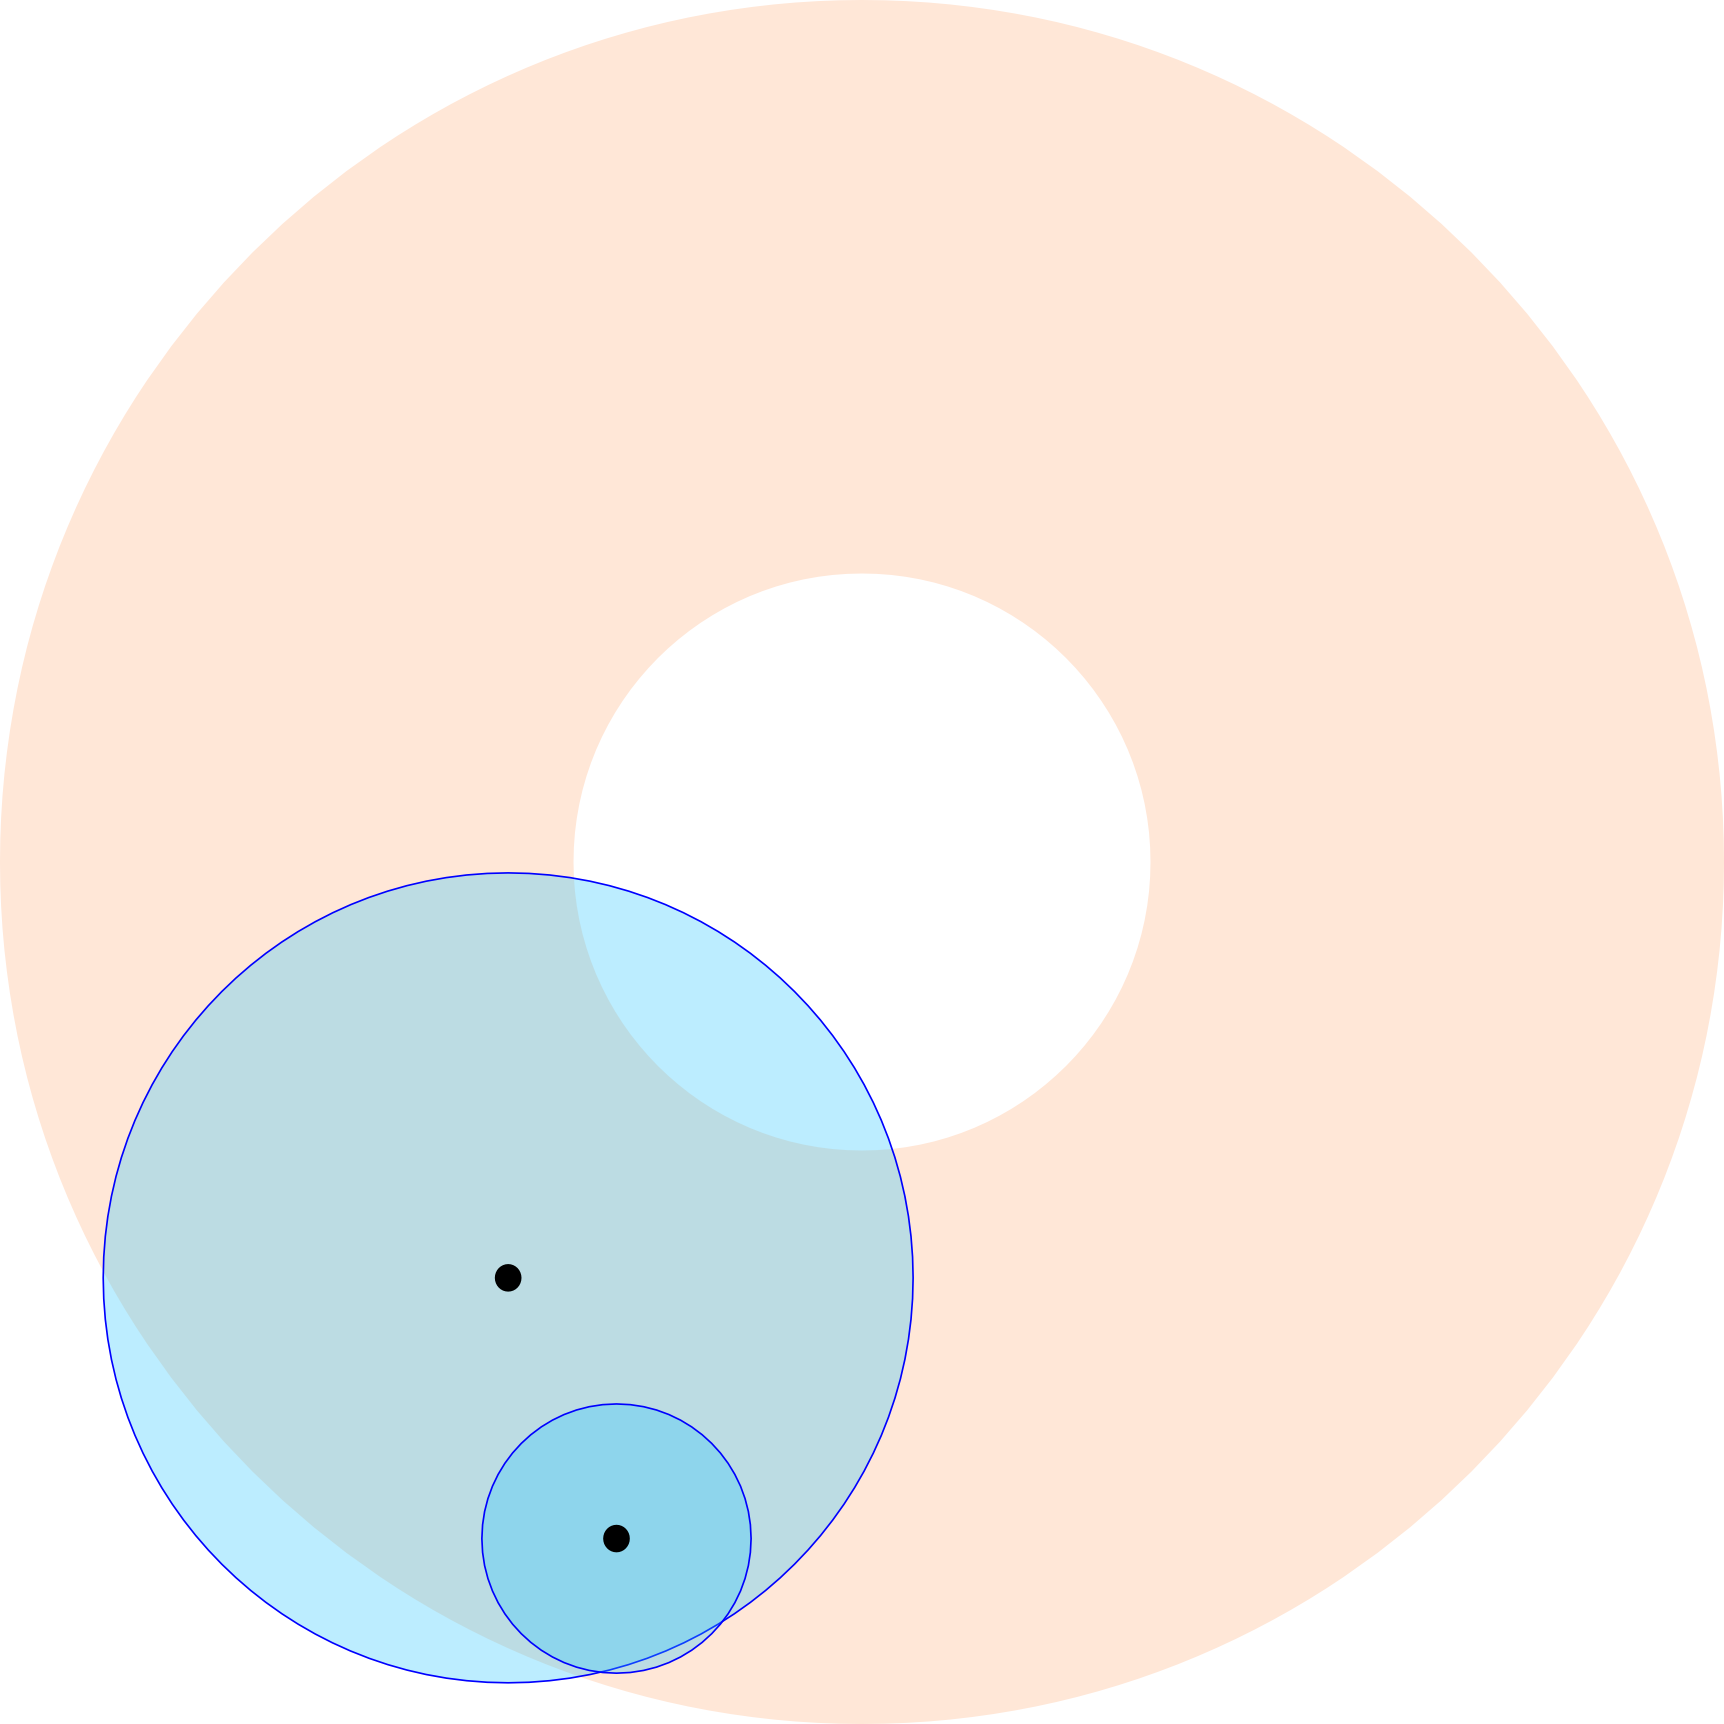
\includegraphics[width=0.5\textwidth]{path5815.png}
\end{frame}%}}}

\begin{frame}\frametitle{Modelo gráfico para el análisis espacial}
%{{{
\centering
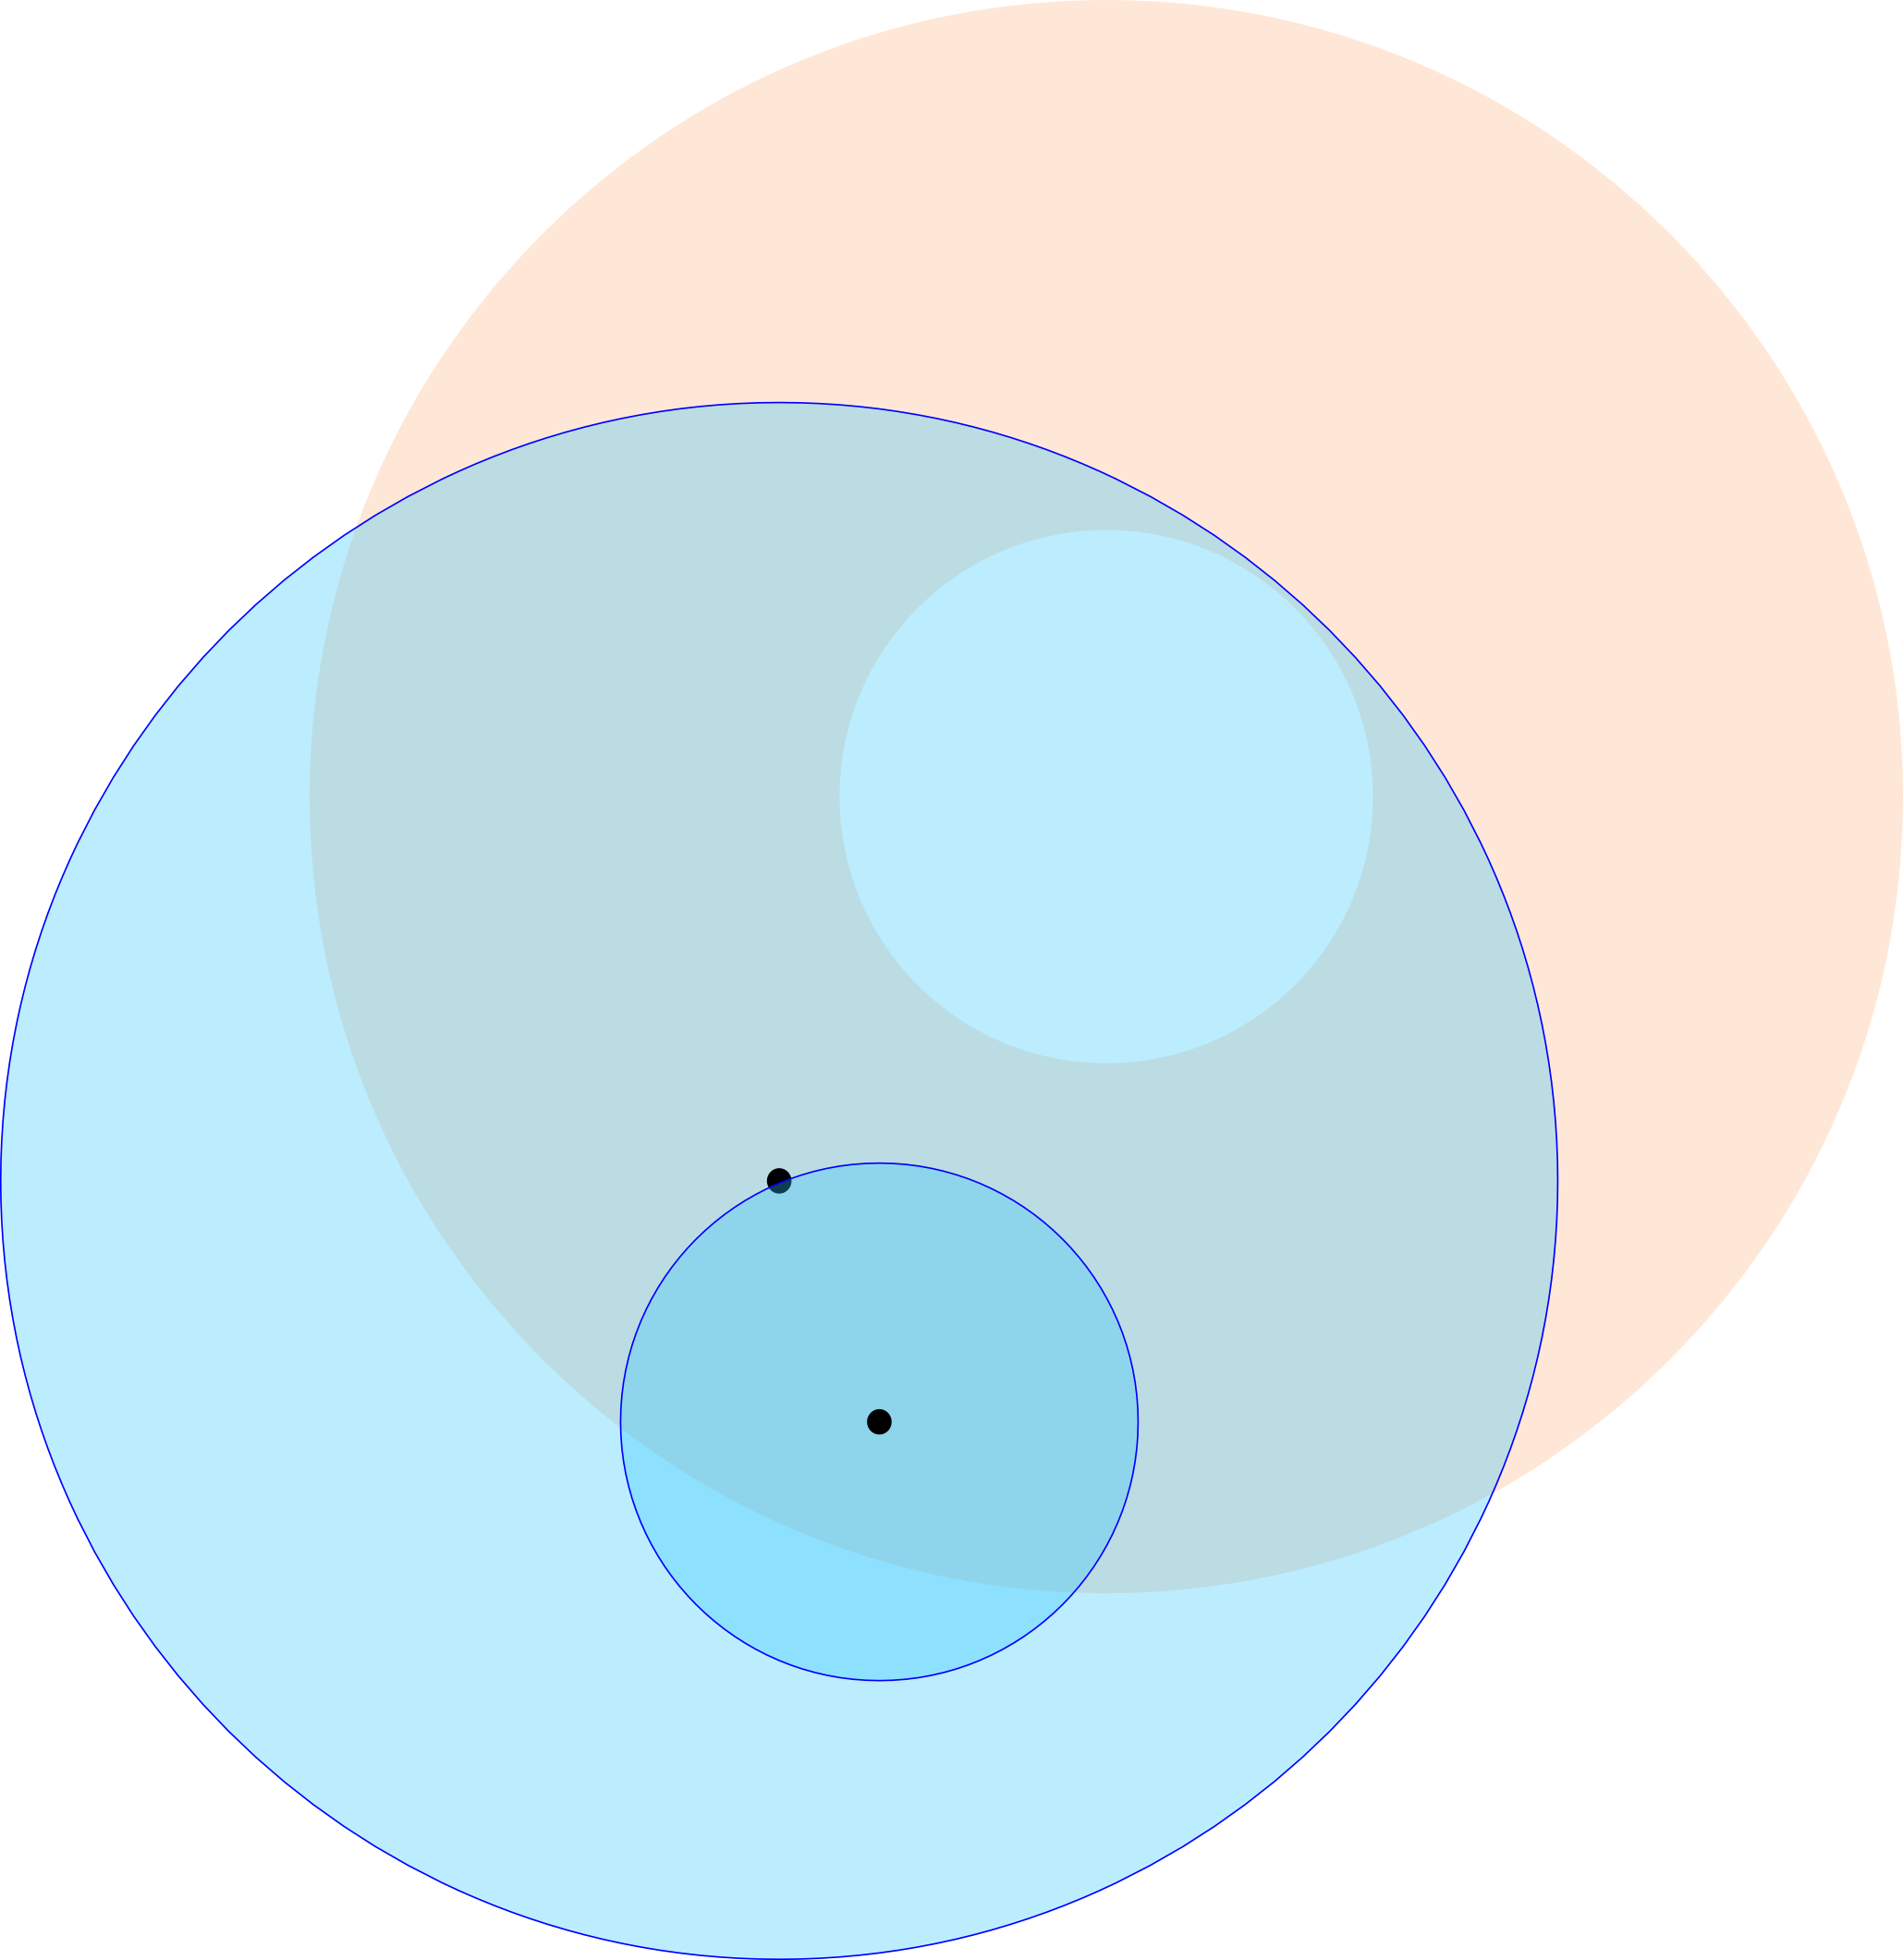
\includegraphics[width=0.5\textwidth]{path5816.png}
\end{frame}%}}}

\begin{frame}\frametitle{Modelo gráfico para el análisis espacial}
%{{{
\centering
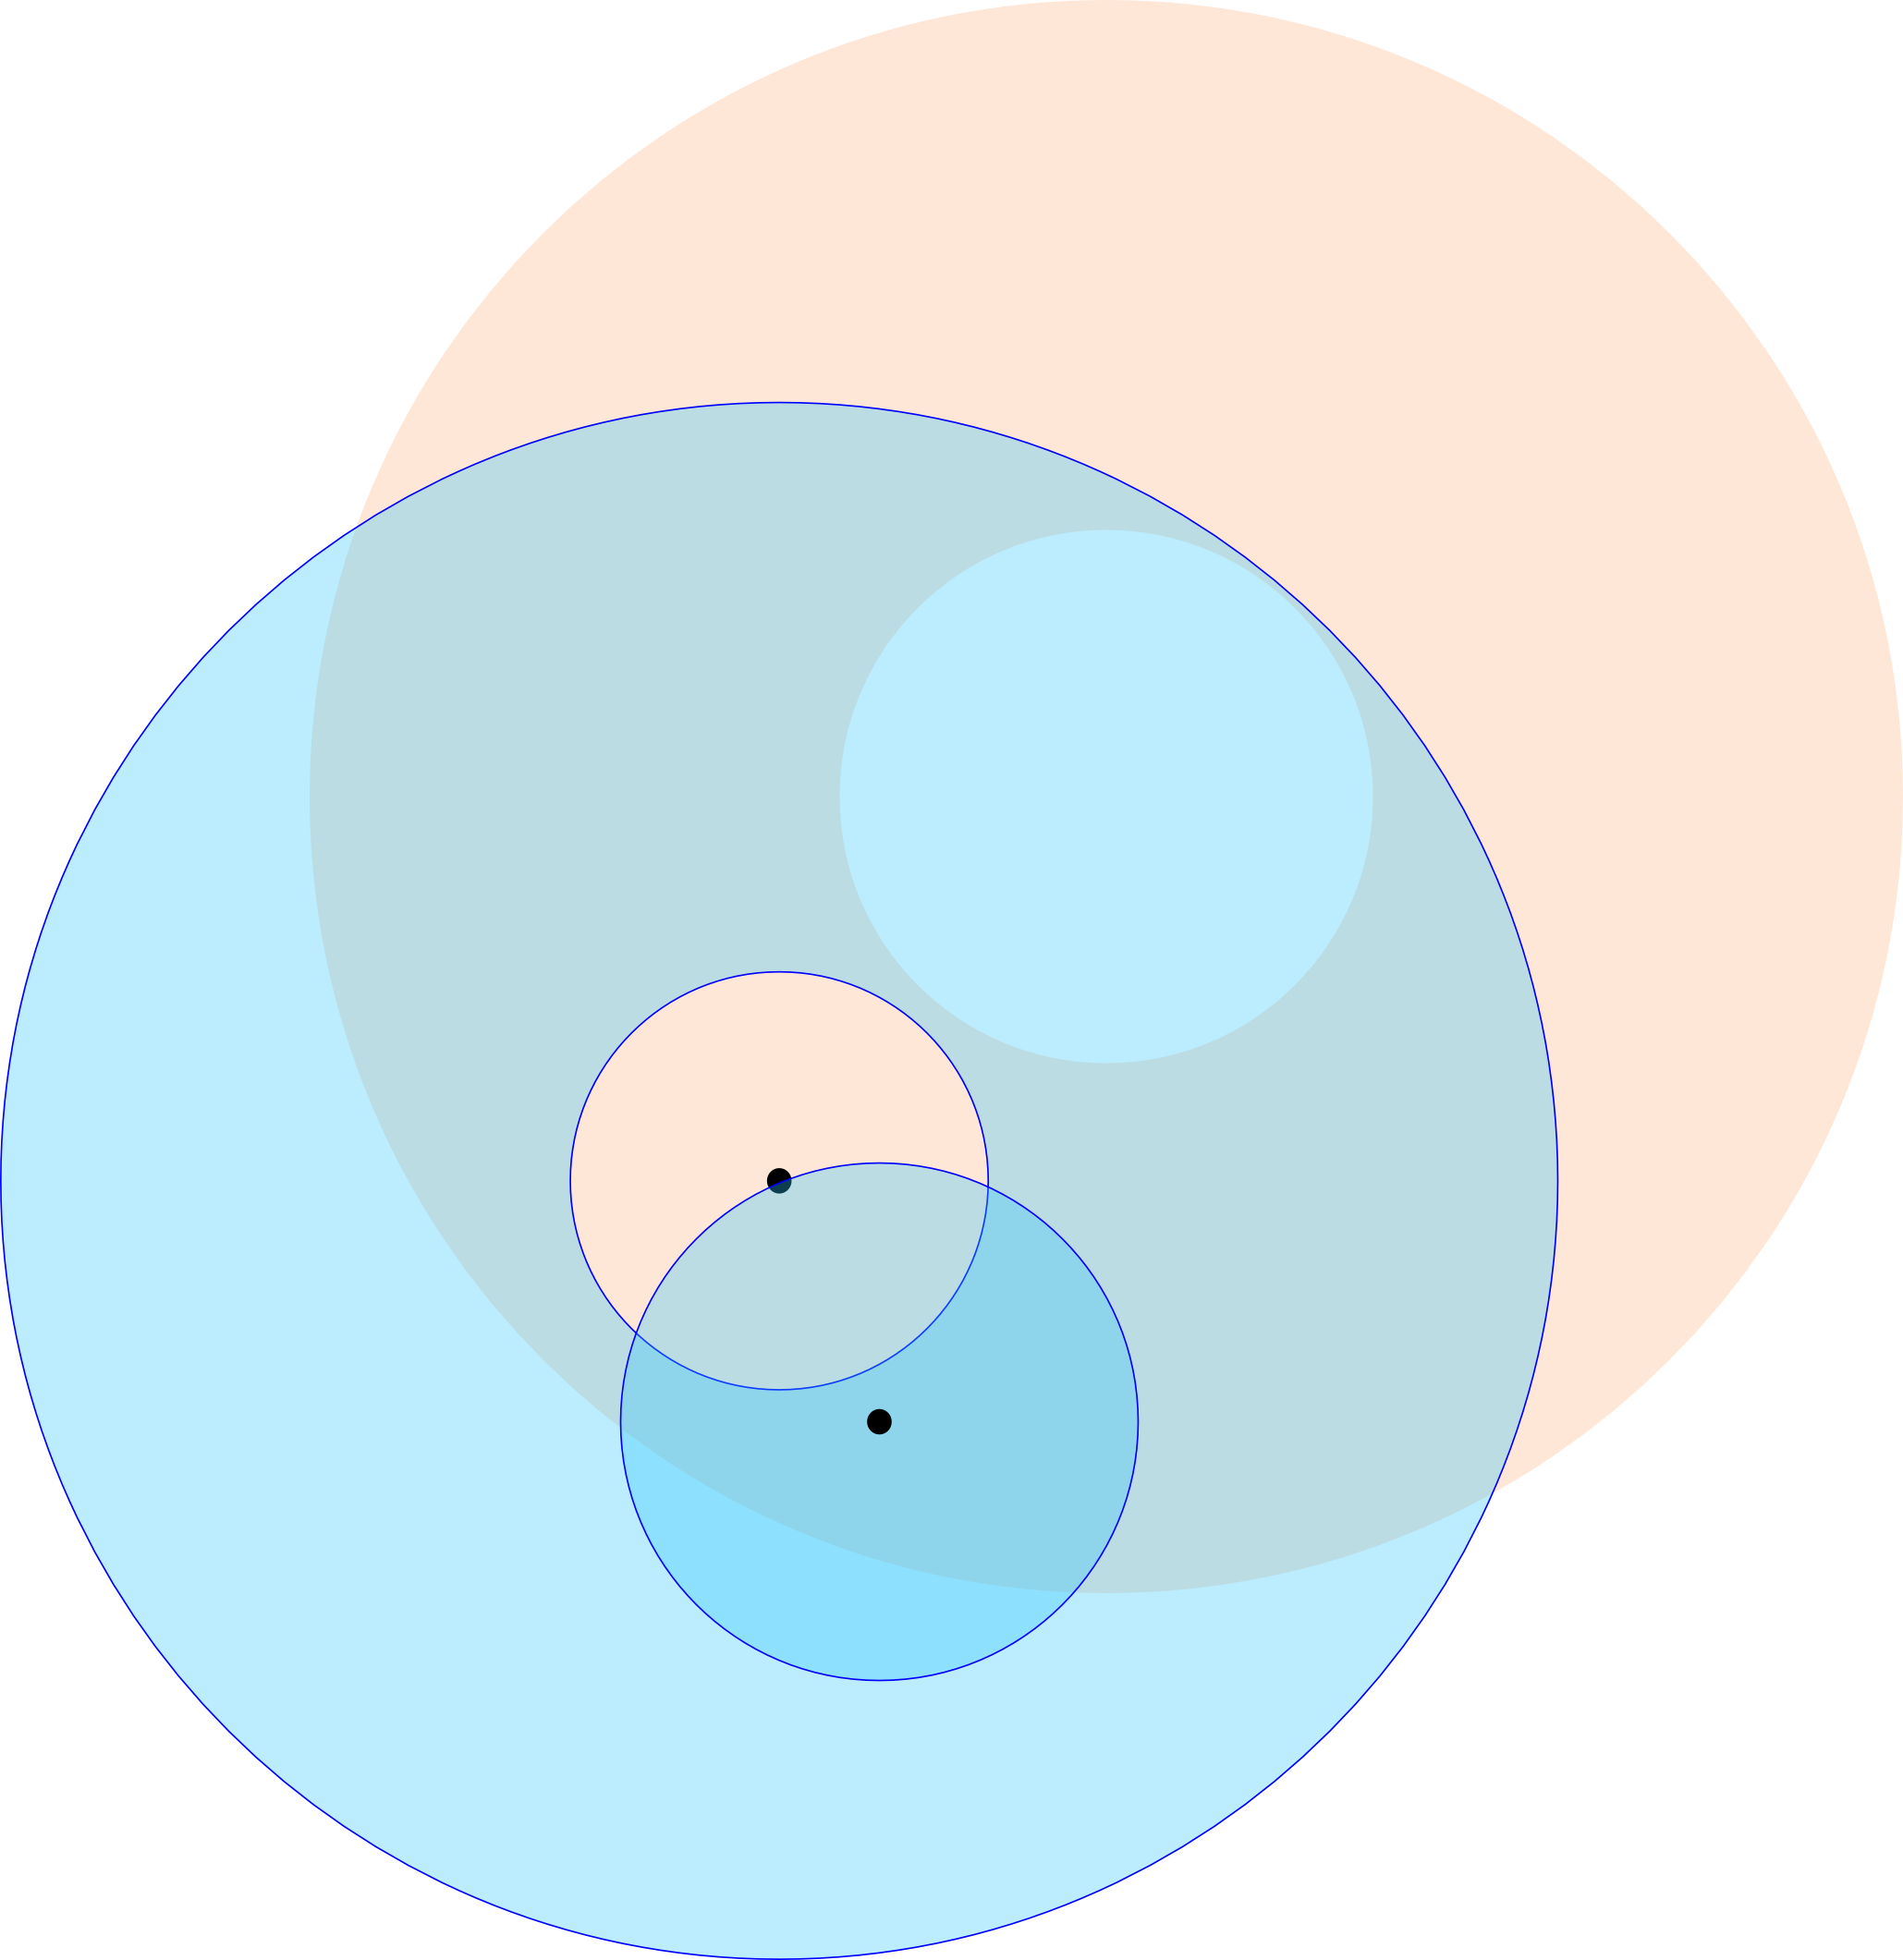
\includegraphics[width=0.5\textwidth]{path5817.png}
\end{frame}%}}}

\begin{frame}\frametitle{Consecuencias para el tiempo de comunicación}
%{{{
Efectos de la disposición espacio--temporal en el tiempo de comunicación
\centering
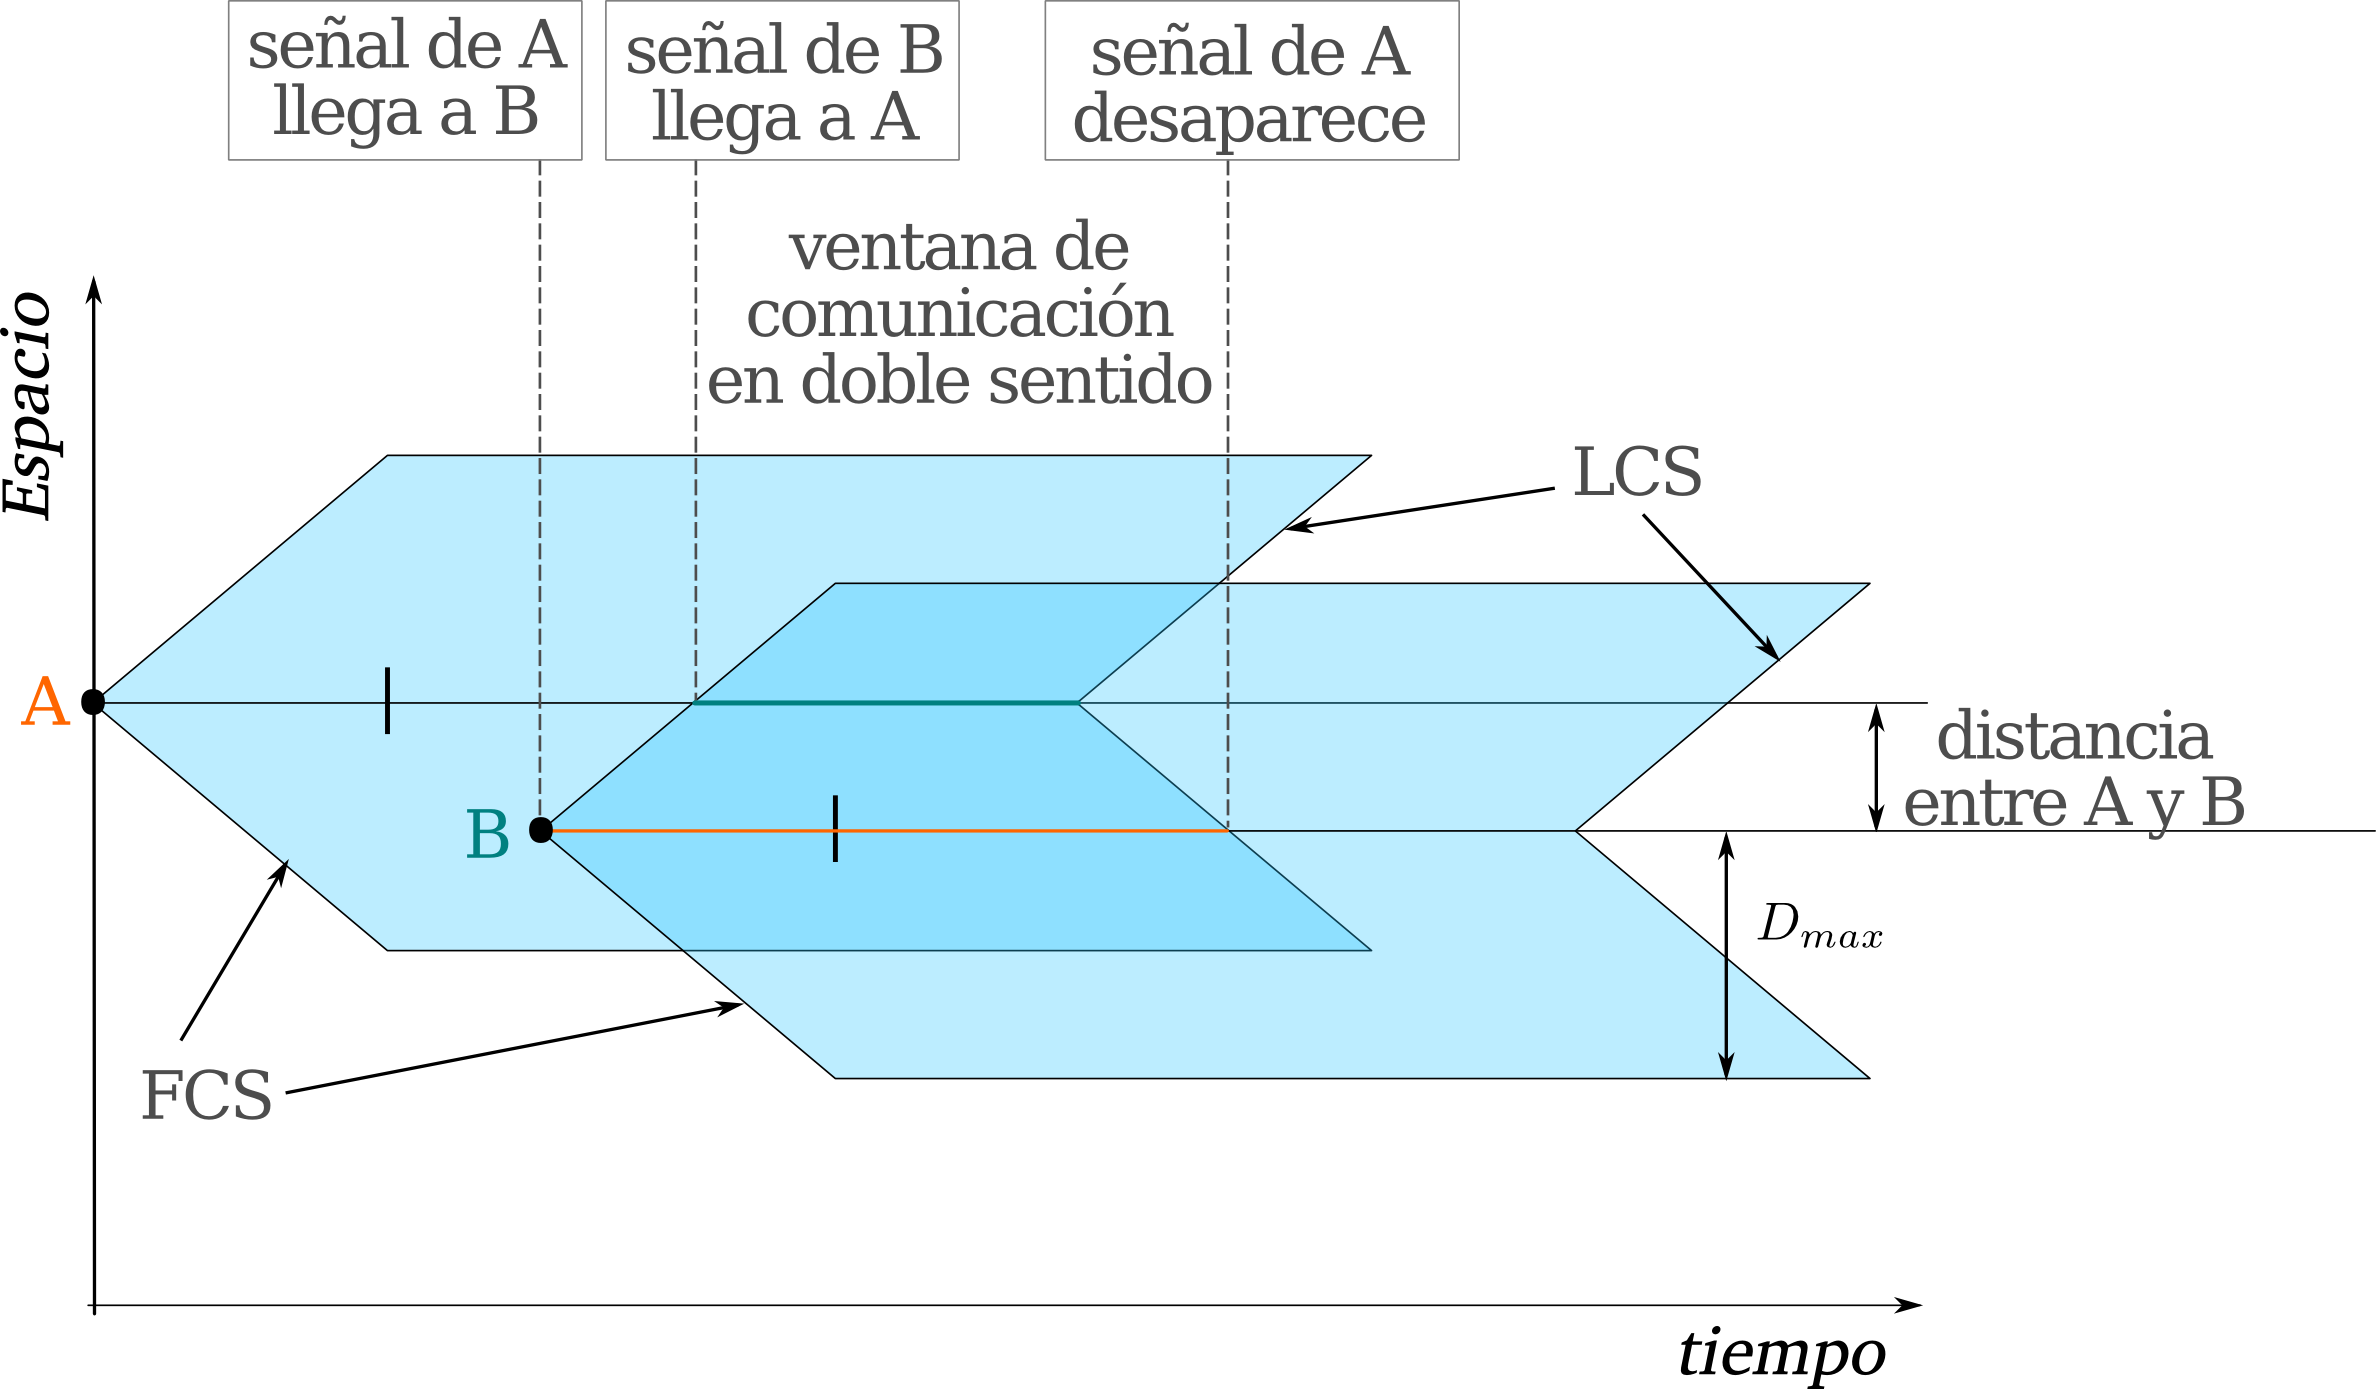
\includegraphics[width=\textwidth]{text4616-5-8-3-4-2.png}
\end{frame}   %}}}

\begin{frame}\frametitle{Consecuencias para el tiempo de comunicación}
%{{{
Efectos de la disposición espacio--temporal en el tiempo de comunicación
\centering
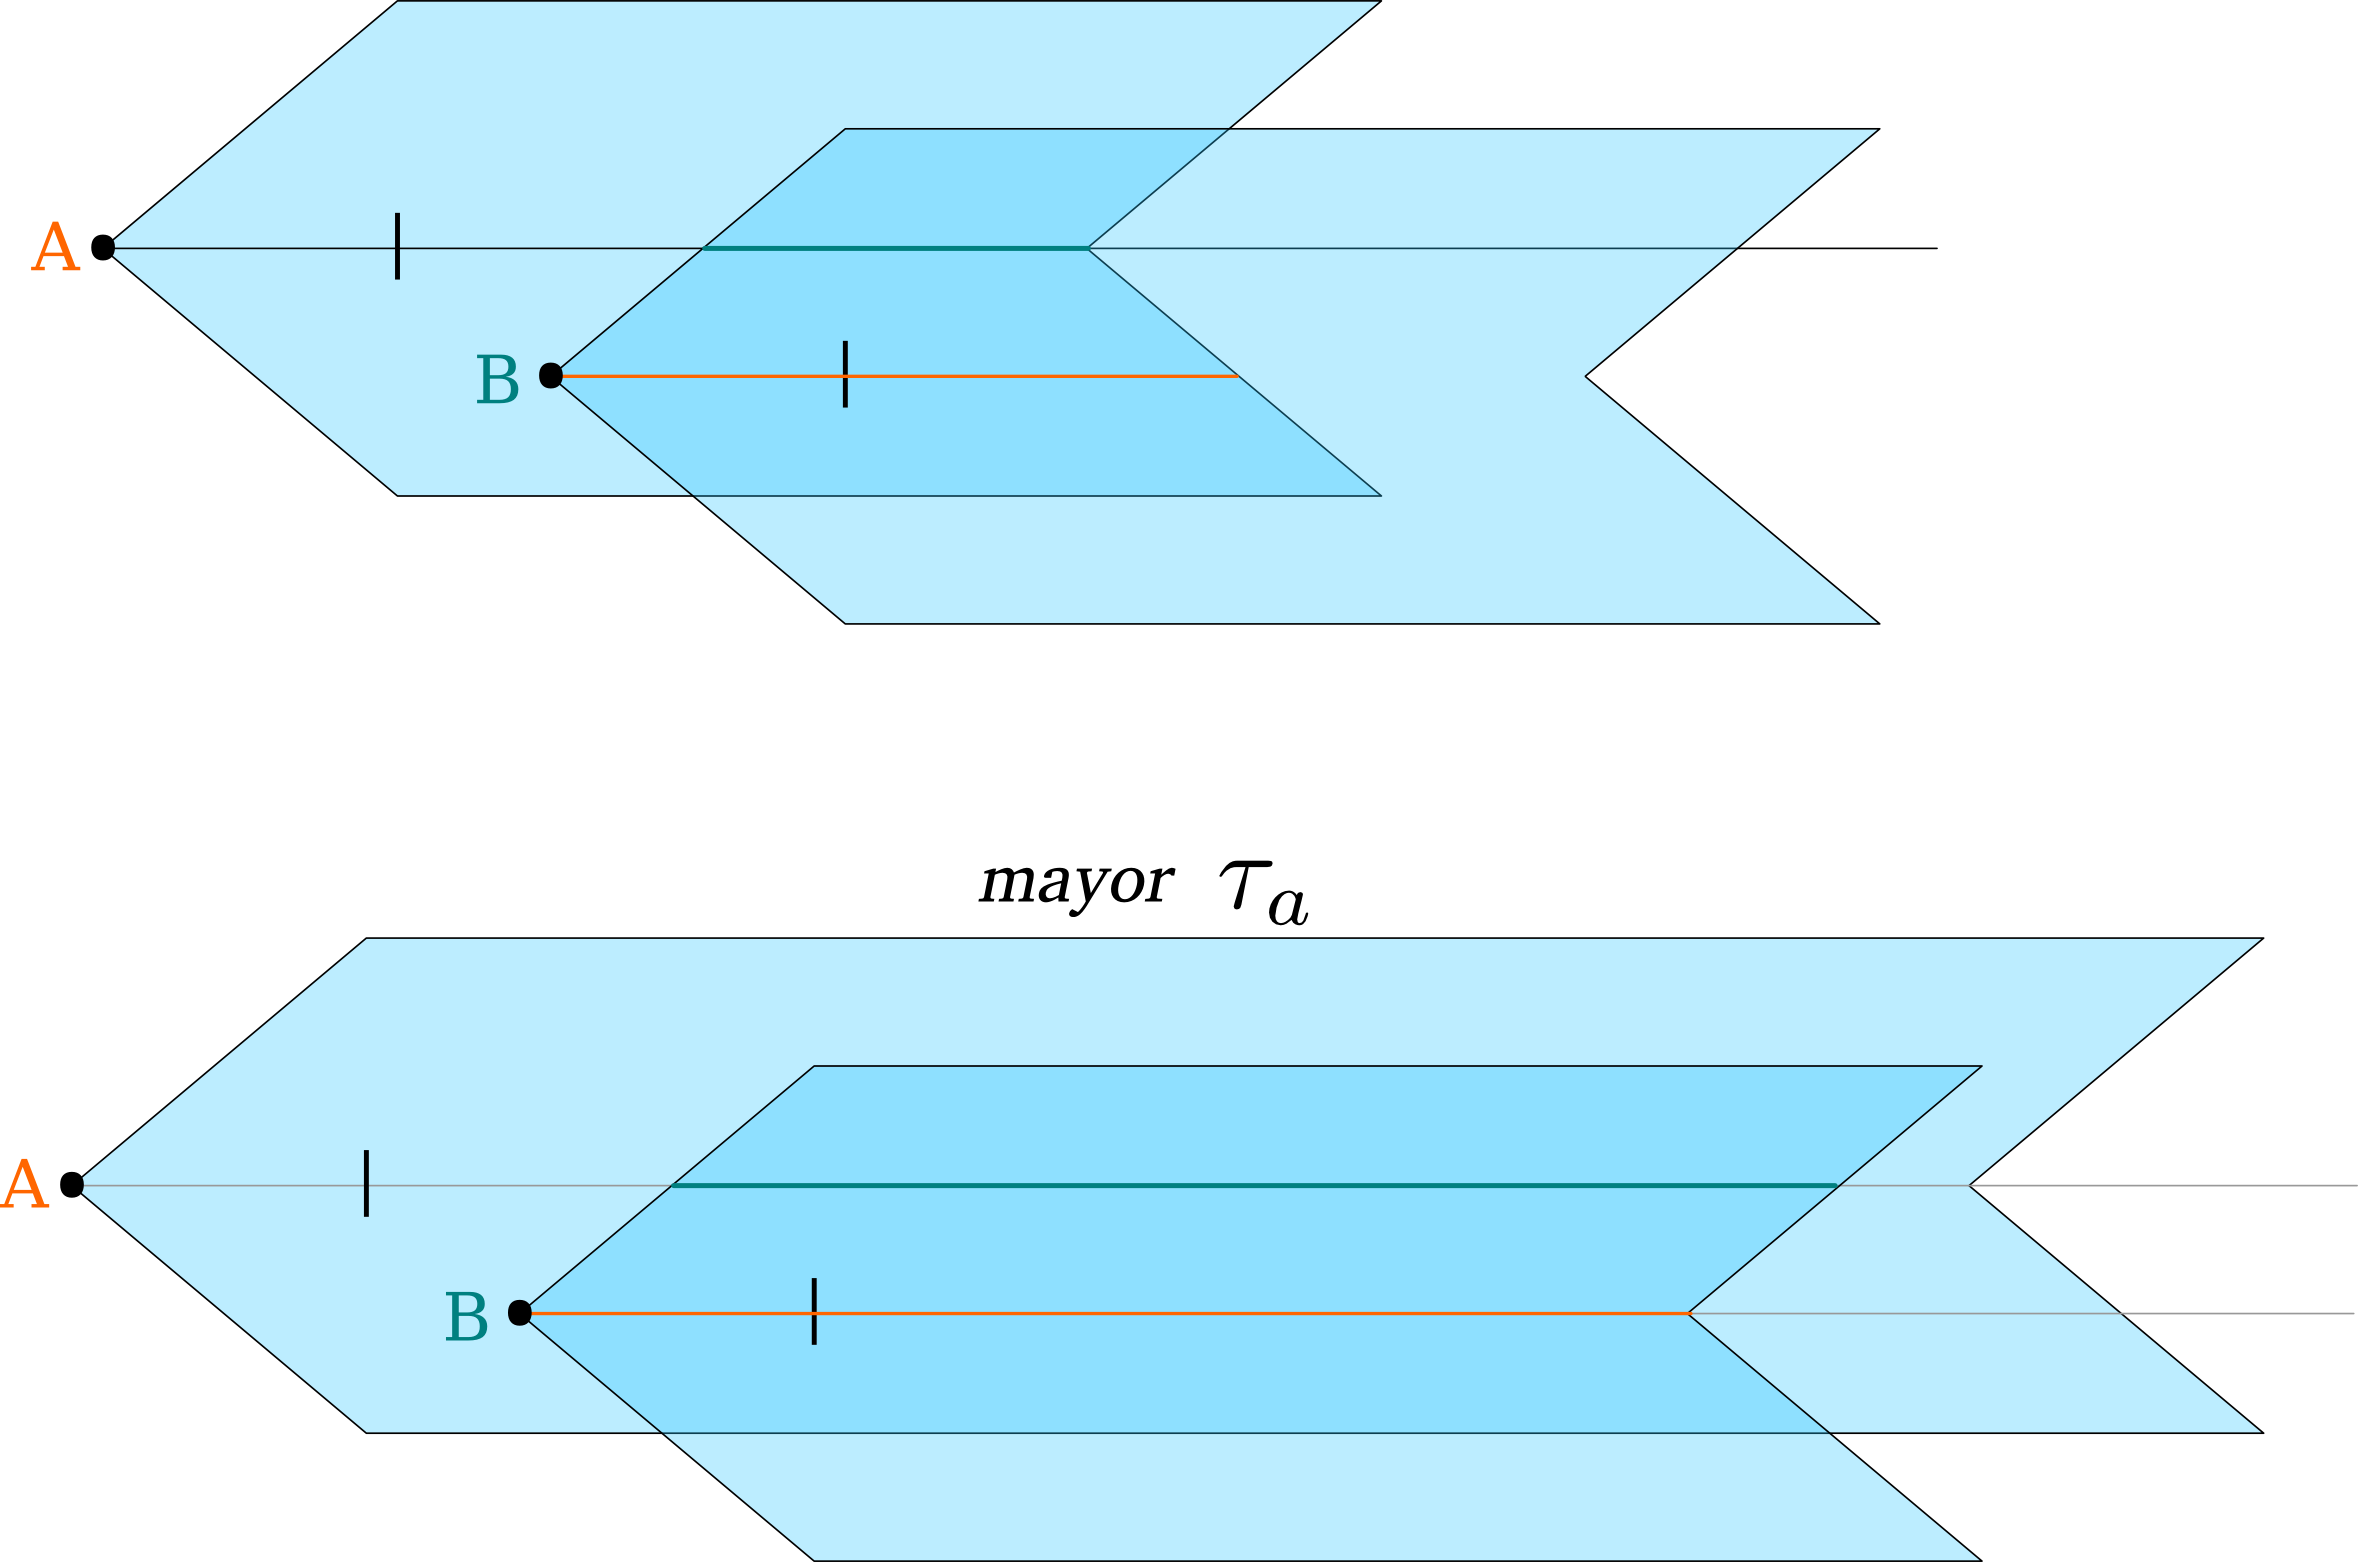
\includegraphics[width=0.9\textwidth]{path9650-0.png}
\end{frame}   %}}}

\begin{frame}\frametitle{Consecuencias para el tiempo de comunicación}
%{{{
Efectos de la disposición espacio--temporal en el tiempo de comunicación
\centering
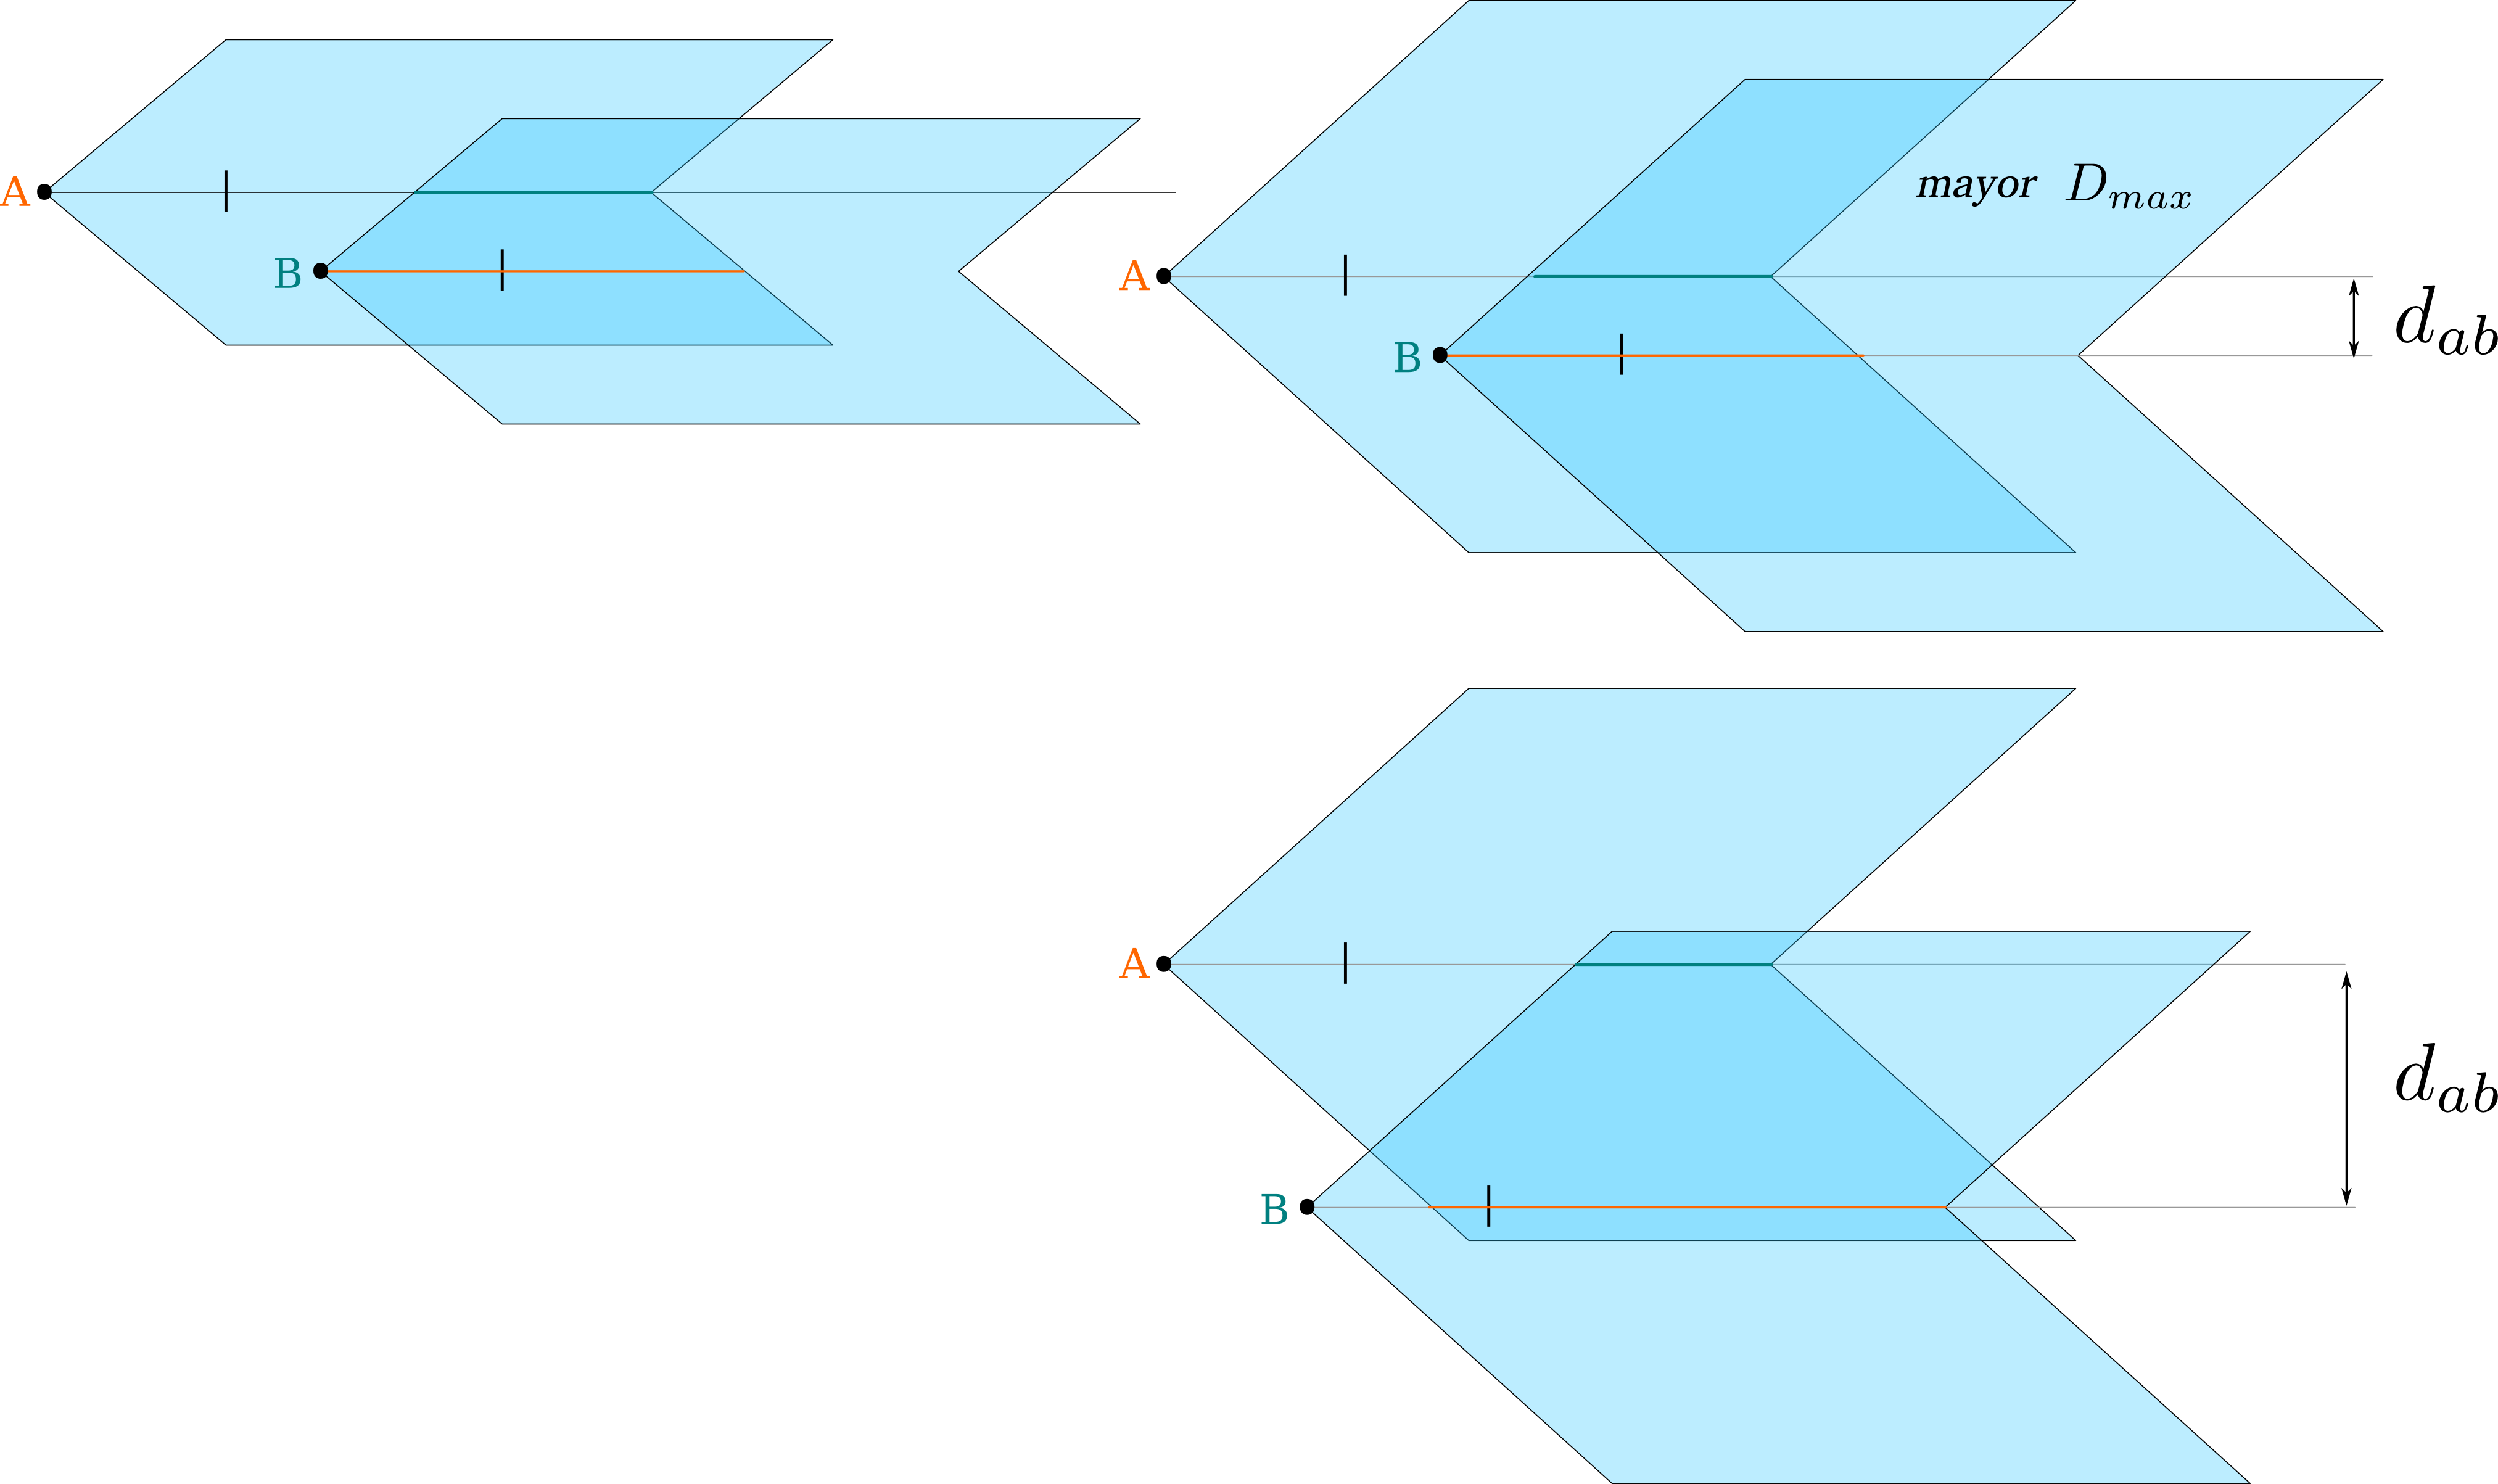
\includegraphics[width=0.9\textwidth]{g10765.png}
\end{frame}   %}}}

%_________________________________________________________________________
\subsection{Aproximación por eventos discretos}

\begin{frame}\frametitle{Selección de eventos}
%{{{

   Se produce un evento cuando:

   \begin{enumerate}
     \item aparece una nueva CETI
     \item desaparece una CETI
     \item una nueva CETI entra en contacto causal
     \item una nueva CETI sale del contacto causal
   \end{enumerate}

\end{frame}  %}}}

\begin{frame}\frametitle{Variables del sistema}
%{{{

   \begin{enumerate}
     \item tiempos de aparición y desaparición de cada CETI
     \item tiempos de primer y último contacto para cada CETI
     \item lista de CETIs activas
   \end{enumerate}

\end{frame}  %}}}
 
\begin{frame}\frametitle{Variables fijas}
%{{{

   \begin{itemize}
      \item Zona habitable galáctica: Se asume simetría radial, está
         definida por los radios mínimos y máximos, medidos en a\~nos
         luz desde el centro de la galaxia.\texttt{GHZ\_inner, GHZ\_outer}
      \item Tiempo medio de vida de una CETI
      \item Tiempo medio que hay que esperar para que surga otra CETI
      \item Distancia máxima a la que puede llegar o recibir un
         mensaje
   \end{itemize}

\end{frame}  %}}}
 
\begin{frame}\frametitle{Variables en el programa}
%{{{

   \begin{itemize}
      \item \texttt{Nact}: Número de CETIs activas
      \item \texttt{Nsee}: Número de contactos por cada CETI
      \item \texttt{Nccc}: CETIs en contacto causal.  Notar que una
         CETI puede tener múltiples contactos de otras CETIs.  Para
         cada una de ellas, guardar:
      \begin{itemize}
         \item \texttt{ID}: ID de la CETI emisora
         \item \texttt{ID}: ID de la CETI receptora
         \item \texttt{t\_hola}: tiempo del primer contacto
         \item \texttt{t\_chau}: tiempo del \'ultimo contacto
      \end{itemize}
   \end{itemize}

\end{frame}  %}}}
% 
%\begin{frame}[fragile]
%%{{{
%\frametitle{Implementaci\'on en el programa}
%
%Para crear la lista de CETIs, usar un diccionario:
%
%\begin{lstlisting}
%d = dict()
%d[12312] = [(3424, 534.35, 565.22)]
%\end{lstlisting}
% 
%las tuplas que se agregan al diccionario son las nuevas CETIs que
%entran en contacto.  En el ejemplo, la CETI con el ID 3424 entra en
%contacto con la CETI 12312 en el tiempo 534.35 y sale del contacto
%causal en el tiempo 565.22.   Para agregar una nueva CETI, 
% 
%\begin{lstlisting}
%ceti = (854, 721.54, 899.14)
%d[12312].append( ceti )
%\end{lstlisting}
%
%\end{frame}%}}}
%
%\begin{frame}\frametitle{Variables derivadas}
%%{{{
%
%   \begin{enumerate}
%     \item Número de contactos unidireccionales
%     \item Número de contactos bidireccionales
%     \item Tiempo de espera hasta el primer contacto
%     \item Duración del contacto
%     \item Número de CETIs activas
%     \item Número de CETIs en contacto causal
%     \item Número de CETIs en contacto simultáneo (con una CETI dada)
%     \item etc.
%   \end{enumerate}
%        
%\end{frame} %}}}
%
% 
%\begin{frame}
%%{{{
%\frametitle{Saltos temporales}
%
%La evolución del sistema se da en saltos temporales.  Los pasos a
%seguir son:
%
%\begin{enumerate}
%   \item identificar el próximo evento, y su tipo
%   \item según el tipo de evento, actualizar las variables del sistema
%   \item actualizar la lista de tiempos de los próximos eventos
%   \item volver a (1)
%\end{enumerate}
%
%\end{frame} %}}}
%             
%            
%
% 
%\begin{frame}
%%{{{
%\frametitle{Saltos temporales}
%
%Para recorrer los eventos discretos, hay que hacer saltos temporales
%de tal forma que entre el tiempo de un evento y el tiempo que sigue no
%hay ningún otro evento.
%
%Para encontrar el tiempo del próximo evento, hay que buscar el mínimo
%de:
%
%\begin{itemize}
%   \item el tiempo de aparición de la próxima CETI (caso 1)
%   \item el tiempo de desaparición de la próxima CETI (caso 2)
%   \item el próximo tiempo en el que se produce un nuevo contacto
%      (caso 3)
%   \item el próximo tiempo en el que desaparece un contacto (caso 4)
%\end{itemize}
%\end{frame}  %}}}
%             
%
% 
%\begin{frame}[fragile]
%%{{{
%\frametitle{Saltos temporales: caso 1}
%
%Llevar una variable que almacene el tiempo de aparición de la próxima
%CETI.
%       
%\begin{lstlisting}
%#Si el proximo evento es de tipo 1:
%
%t_this_active = t_now + np.random.exponential(t_mean_wait, 1) 
%t_WakeUp_next = min( t_this_active, t_WakeUp_next )
%
%\end{lstlisting}       
%
%\end{frame}   %}}}
%                    
%
%\begin{frame}[fragile]
%%{{{
%\frametitle{Saltos temporales: caso 2}
%
%Llevar una variable que almacene el tiempo de desaparición de la próxima
%CETI.
%       
%\begin{lstlisting}
%#Si el proximo evento es de tipo 2:
%
%t_GoDown_next = t_now + np.random.exponential(t_mean_active, 1)
%
%\end{lstlisting}       
%
%\end{frame} %}}}
%                    
 



\begin{frame}\frametitle{Caso 1: aparece una nueva CETI}
%{{{
   \centering
   
\includegraphics[width=0.75\textwidth]{C1.png}
\end{frame}  %}}}

\begin{frame}\frametitle{Caso 1: aparece una nueva CETI}
%{{{

   Modificaciones al estado del sistema:
   \begin{itemize}
      \item Agregar la CETI ``A'' a la lista de CETIs activas
      \item Sortear la duración de la actividad de comunicación de la
         CETI ``A''
      \item Sortear el intervalo de tiempo hasta la aparición de la
         próxima CETI: \texttt{t\_WakeUp\_next}
      \item Agregar la CETI ``A'' al árbol
      \item Identificar todas las CETIs que están a menos de $D_{max}$
         de la nueva CETI, y actualizar la lista de tiempos
   \end{itemize}

\end{frame}  %}}}
 
\begin{frame}\frametitle{Caso 2: desaparece una CETI}
%{{{
   \centering
   
\includegraphics[width=0.75\textwidth]{C2.png}
\end{frame}  %}}}

\begin{frame}\frametitle{Caso 2: desaparece una CETI}
%{{{

   Modificaciones al estado del sistema:
   \begin{itemize}
      \item Eliminar la CETI a la lista de CETIs activas
   \end{itemize}

\end{frame}  %}}}

%\begin{frame}\frametitle{Caso 3: se alcanza la máxima distancia de contacto}
%%{{{
%   \centering
%   
\includegraphics[width=0.75\textwidth]{C3.png}
%
%\end{frame}  %}}}
%
%\begin{frame}\frametitle{Caso 3: se alcanza la máxima distancia de contacto}
%%{{{
%
%   Modificaciones al estado del sistema:
%   \begin{itemize}
%      \item Marcar la CETI A para que la máxima distancia de contacto
%         esté limitada
%   \end{itemize}
%
%\end{frame}  %}}}

\begin{frame}\frametitle{Caso 3: una nueva CETI entra en contacto causal}
%{{{
   \centering
   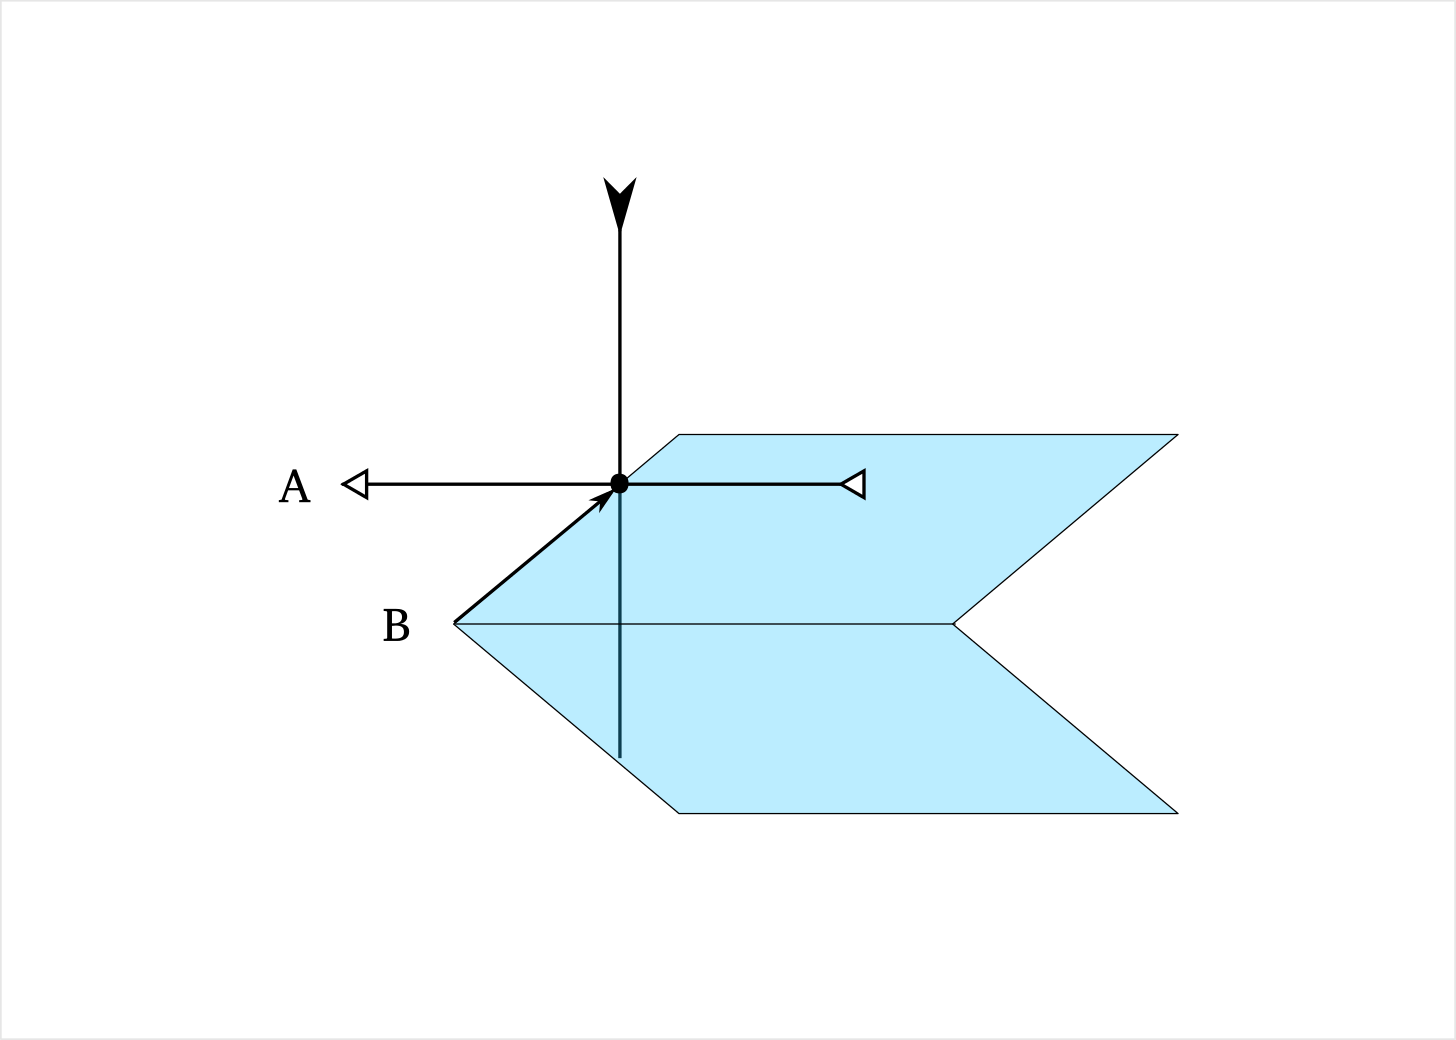
\includegraphics[width=0.75\textwidth]{C4.png}
\end{frame}  %}}}

\begin{frame}\frametitle{Caso 3: una nueva CETI entra en contacto causal}
%{{{

   Modificaciones al estado del sistema:
   \begin{itemize}
      \item  Agregar la CETI B a la lista de contactos de la CETI A
   \end{itemize}

\end{frame}  %}}}

\begin{frame}\frametitle{Caso 4: una nueva CETI sale del contacto causal}
%{{{
   \centering
   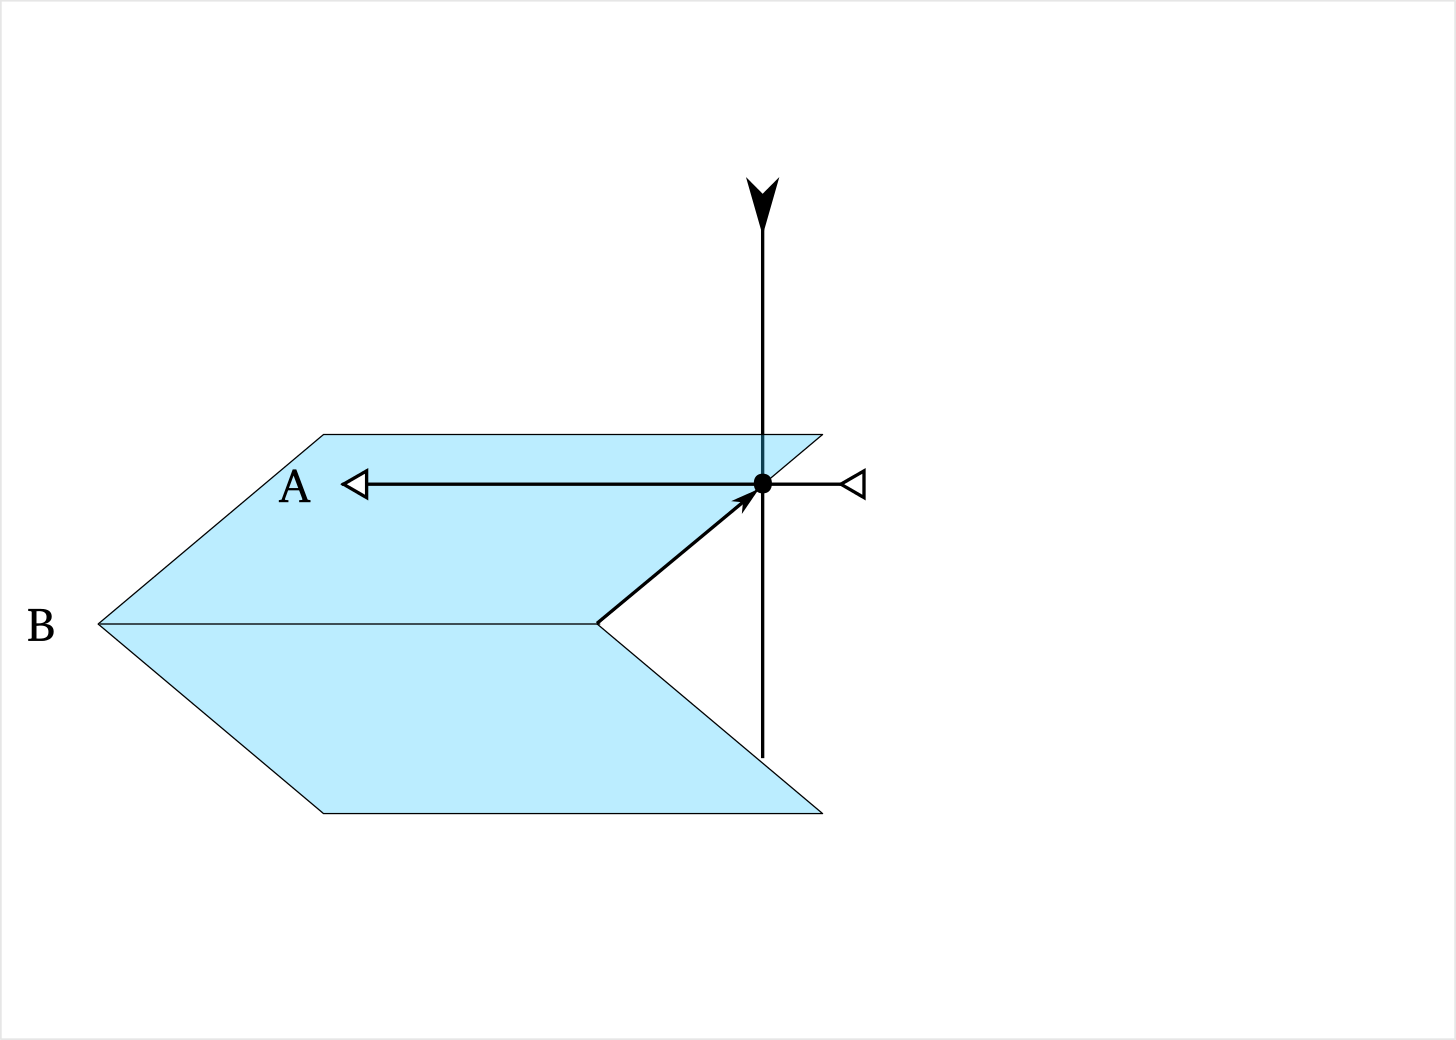
\includegraphics[width=0.75\textwidth]{C5.png}
\end{frame}  %}}}

\begin{frame}\frametitle{Caso 4: una nueva CETI sale del contacto causal}
%{{{

   Modificaciones al estado del sistema:
   \begin{itemize}
      \item 
   \end{itemize}

\end{frame}  %}}}

\begin{frame}\frametitle{Búsqueda del siguiente evento}
%{{{

   Construir una lista de saltos temporales:

   \begin{itemize}
      \item 
   \end{itemize}

\end{frame}  %}}}
 
\begin{frame}\frametitle{Discusión}
%{{{
   \begin{itemize}
      \item Código en progreso
      \item Lenguaje: python
      \item Accesible via GitHub
      \item Modificaciones al plan de trabajo?
      \item Colaboradores?
      \item Reuniones de trabajo y/o difusión de resultados?
   \end{itemize}
\end{frame}%}}}






\begin{frame}\frametitle{Output}
%{{{

La salida de la simulación está guardad en una variable llamada CETI.

La misma es una lista de objetos que son también listas.

El elemento cero de cada lista (i.e., cada elemento de CETI) contiene:

\begin{itemize}
   \item coordenada X
   \item coordenada Y
   \item tiempo de inicio de la capacidad de comunicaci\'on
   \item tiempo de final de la capacidad de comunicaci\'on
\end{itemize}

y los demás elementos contienen:
 
\begin{itemize}
   \item coordenada X de la CETI
   \item coordenada Y de la CETI
   \item tiempo del primer contacto
   \item tiempo del \'ultimo contacto
\end{itemize}
 

\end{frame}%}}}

 
\begin{frame}\frametitle{Resultados cuantitativos de la simulaci\'on}
%{{{

\begin{itemize}
   \item distribucion del numero de contactos
   \item distribucion de la duracion de los contactos
   \item distribucion del tiempo que hay que esperar para el proximo contacto
\end{itemize}
 

\end{frame}%}}}
                               


\end{document}
